\chapter{Empirical Analysis}

This chapter is structured as such: a first section describes the data and its
variables, their source and a reason to incorporate them in the analysis. This
is followed by a presentation of the results and their analysis.

\section{Data}

The main data comes from the OECD Economic Outlook ($98^{th}$ edition)
(cf. \cite{oecd2015eo}) with annual and quarterly frequency. We only use a
subset of the data set with the following variables.
\begin{itemize}
\item Public employment rate of OECD countries between 1990 to 2012. Public
  employment rate is defined as the number of civil servant divided by the
  total labor force. Figure \ref{fig:egr} shows the public employment rate used
  for the data analysis.
\item Unemployment rate in percent. Everything else being equal, the
  correlation with public employment rate should be negative: the total labor
  force is composed of employed plus unemployed people, hence if the number of
  workers in the private industry remain stable, a diminishing unemployment
  rate should increase the public employment rate.
\item Government revenues in percent of GDP: the share of GDP that the
  government receive from taxes and others sources of income. This variable
  captures the size of the government.
\item Net lending in percent of GDP: the difference between revenues and
  expenditures scaled by GDP. The net lending captures how well the incumbent
  government manages its budget.
\item GDP Growth in percent. It is believed that this variable represent the
  effect economic cycle and momentum in an economy.
\item GDP per capita in 2010 USD Purchasing power parity, in order to control
  for the Wagner's Law, stating that richer populations care more about common
  goods (often provided by government). The effect of wealth over the public
  employment share should be non-linear, reason for which its $\log$ is used in
  the models.
\end{itemize}

Moreover, the following time series have been collected to test the assertion
of the literature.
\begin{itemize}
\item The 105 election quarters for the relevant OECD countries were recorded
  from Wikipedia (\cite{wiki2015election}); From the election dates, one can
  deduce the number of years until the normal end of the term.
\item Fiscal transparency score, \cite{wang2015trends} from the IMF. A low
  fiscal transparency allows governments to use windfall revenues to boost the
  number of public employees or to adjust their national accounts.
\item Political direction of the executive government (left or right) from the
  World Bank (\cite{beck2001new}). One desires to capture the effect or
  correlation of the political partisanship over public employment rate. It
  should be increased when a left-wing governments is elected.
\item Gini coefficient, before and after tax from the Standardizing the world
  income inequality database (\cite{solt2009standardizing}). The Gini
  coefficient is a standard measure to assess the income inequality within a
  country. A high level of inequality should lead to a bigger rate of public
  employees, as a mean for the government to redistribute wealth.
\end{itemize}

Plots of these variable are showed in Appendix \ref{ch:data-viz}. We also
assumed that structural breaks could have affected the public employment rate
in the data set. \cite{james2014ecp} provides a non-parametric algorithm to
detect such point. As Figure \ref{fig:strct:breaks} depicts, although there are
some individual changes, there are no overall break at given time point. Hence
the idea has been abandoned.

\section{Analysis}

\subsection{Results}

For our analysis, we extend the model from Equation \eqref{eq:reg} with the
following equation:
\begin{align*}
  Y_{it} = \alpha Y_{i{t-1}} + X_{it}\beta + \eta_i + \tau_t +
  \varepsilon_{it} \quad i \in \{1, \dots, n\},\ t \in \{1, \dots, T\},
\end{align*}
where $X_{it}$ is the independent variable and contains the unemployment rate,
government revenues and net lending for $i$-th country at time $t$. The other
variables are similar to Equation \eqref{eq:reg}. This model, albeit
counter-intuitive, is stable and robust. Additionally, the auto-regressive
aspect reduces the correlation of the error terms $\varepsilon_{it}$.  Table
\ref{tbl:main-coeff} shows the coefficient of the regression\footnote{The
  output of linear models has produced with the Stargazer package
  (\cite{hlavac2015stargazer}) used with the statistical programming language
  \textsf{R}.}. Moreover, Figure \ref{fig:diag:lm} provides some support about
the soundness of our statistical model: the residuals of the regression seem to
be uncorrelated, although there is evidence they do not follow a Gaussian
distribution. The regression tables for the additional variables are in the
Appendix \ref{ch:reg-tbls}.  Note the following supplementary observations.


\begin{enumerate}
\item The number of fitted parameter is much bigger than what is displayed in
  the tables: one degree of freedom is allocated for each quarter to fit $\tau_t$
  (88 for the 22 years of observations) and for the country parameter $\eta_i$
  (17 parameters).
\item The main variables (unemployment rate, government revenue and net
  lending) keep the same regression coefficient and their statistical
  significance.
\item The absolute size of these coefficients are quite small.
\item GDP growth and the Gini coefficient after taxes have significant
  regression coefficient before adjustment of the $p$-values, but become
  insignificant afterwards.
\item The effect of the wealth of a nation, measured by the GDP per capita, is
  unexpectedly not correlated. This observation does not support the Wagner's
  law.
\item Unfortunately, the number of years before the next official election, the
  left-wing partisanship, the fiscal transparency do not seem to influence the
  public employment rate, contradicting literature.
\end{enumerate}

\subsection{Robustness analysis}

The coefficients of the base model remain stable and significant when
additional indepedent variables are added. The same holds when the frequency is
lowered to annual data as well. Furthermore, interaction terms have also been
introduced in the robustness tests, without creating major modifications to our
previous finding.

Note that for the robustness analysis, missing data lead to a different number
of observations as input for the model, making the comparison more difficult.

One of the additional difficulty in this analysis is that country means are
sufficient to predict the values of the public employment rate: Variations are
small with a high autocorrelation coefficient. In order to tackle this problem,
we tried to fit the time-difference of the public employment rate, but the
explained variance (commonly known as the $R^2$) is negligible (about $9\%$
with an over-fitting model).

In short, unemployment rate, government revenues and net lending compose a
statistically sound and robust model to explain the public employment
rate. Unfortunately, according to the data, other variables, such as fiscal
transparency, the remaining years until the end of the government mandate or
measure of inequality do not offer additional information.


\begin{landscape}
  \begin{figure}[!ht] \centering
    % Created by tikzDevice version 0.9 on 2016-01-12 01:24:47
% !TEX encoding = UTF-8 Unicode
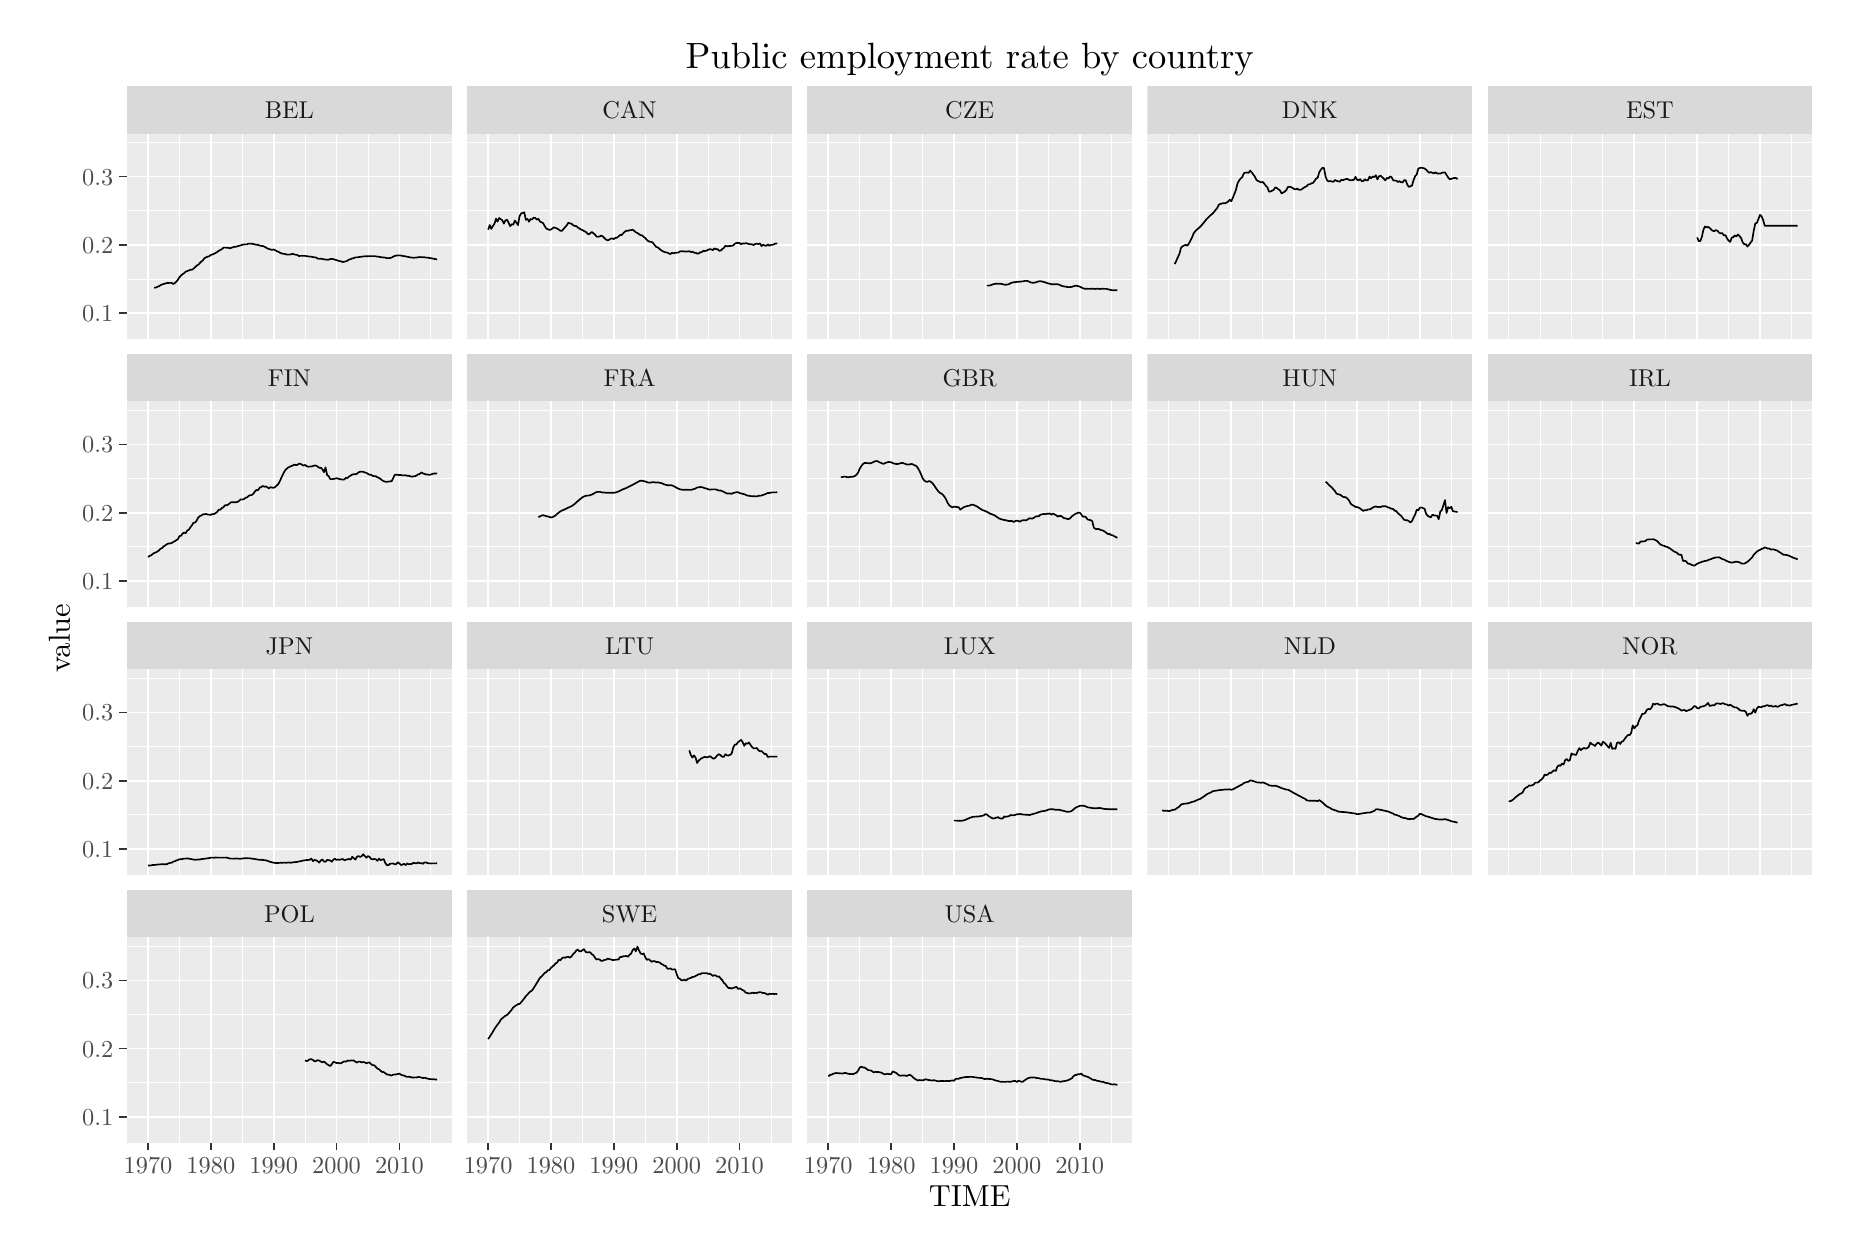
\begin{tikzpicture}[x=1pt,y=1pt]
\definecolor{fillColor}{RGB}{255,255,255}
\path[use as bounding box,fill=fillColor,fill opacity=0.00] (0,0) rectangle (650.43,433.62);
\begin{scope}
\path[clip] (  0.00,  0.00) rectangle (650.43,433.62);
\definecolor{drawColor}{RGB}{255,255,255}
\definecolor{fillColor}{RGB}{255,255,255}

\path[draw=drawColor,line width= 0.6pt,line join=round,line cap=round,fill=fillColor] (  0.00,  0.00) rectangle (650.43,433.62);
\end{scope}
\begin{scope}
\path[clip] ( 35.87,321.12) rectangle (153.28,395.37);
\definecolor{fillColor}{gray}{0.92}

\path[fill=fillColor] ( 35.87,321.12) rectangle (153.28,395.37);
\definecolor{drawColor}{RGB}{255,255,255}

\path[draw=drawColor,line width= 0.3pt,line join=round] ( 35.87,342.80) --
	(153.28,342.80);

\path[draw=drawColor,line width= 0.3pt,line join=round] ( 35.87,367.46) --
	(153.28,367.46);

\path[draw=drawColor,line width= 0.3pt,line join=round] ( 35.87,392.11) --
	(153.28,392.11);

\path[draw=drawColor,line width= 0.3pt,line join=round] ( 54.83,321.12) --
	( 54.83,395.37);

\path[draw=drawColor,line width= 0.3pt,line join=round] ( 77.54,321.12) --
	( 77.54,395.37);

\path[draw=drawColor,line width= 0.3pt,line join=round] (100.25,321.12) --
	(100.25,395.37);

\path[draw=drawColor,line width= 0.3pt,line join=round] (122.96,321.12) --
	(122.96,395.37);

\path[draw=drawColor,line width= 0.3pt,line join=round] (145.67,321.12) --
	(145.67,395.37);

\path[draw=drawColor,line width= 0.6pt,line join=round] ( 35.87,330.48) --
	(153.28,330.48);

\path[draw=drawColor,line width= 0.6pt,line join=round] ( 35.87,355.13) --
	(153.28,355.13);

\path[draw=drawColor,line width= 0.6pt,line join=round] ( 35.87,379.78) --
	(153.28,379.78);

\path[draw=drawColor,line width= 0.6pt,line join=round] ( 43.48,321.12) --
	( 43.48,395.37);

\path[draw=drawColor,line width= 0.6pt,line join=round] ( 66.19,321.12) --
	( 66.19,395.37);

\path[draw=drawColor,line width= 0.6pt,line join=round] ( 88.90,321.12) --
	( 88.90,395.37);

\path[draw=drawColor,line width= 0.6pt,line join=round] (111.61,321.12) --
	(111.61,395.37);

\path[draw=drawColor,line width= 0.6pt,line join=round] (134.32,321.12) --
	(134.32,395.37);
\definecolor{drawColor}{RGB}{0,0,0}

\path[draw=drawColor,line width= 0.6pt,line join=round] ( 45.75,339.57) --
	( 46.31,339.73) --
	( 46.88,339.95) --
	( 47.45,340.22) --
	( 48.02,340.56) --
	( 48.59,340.82) --
	( 49.15,341.01) --
	( 49.72,341.16) --
	( 50.29,341.33) --
	( 50.86,341.37) --
	( 51.42,341.40) --
	( 51.99,341.42) --
	( 52.56,341.00) --
	( 53.13,341.31) --
	( 53.70,341.83) --
	( 54.26,342.50) --
	( 54.83,343.42) --
	( 55.40,344.05) --
	( 55.97,344.54) --
	( 56.53,344.90) --
	( 57.10,345.45) --
	( 57.67,345.66) --
	( 58.24,345.89) --
	( 58.81,346.16) --
	( 59.37,346.13) --
	( 59.94,346.56) --
	( 60.51,347.06) --
	( 61.08,347.63) --
	( 61.64,347.96) --
	( 62.21,348.56) --
	( 62.78,349.12) --
	( 63.35,349.58) --
	( 63.91,350.37) --
	( 64.48,350.64) --
	( 65.05,350.86) --
	( 65.62,351.03) --
	( 66.19,351.50) --
	( 66.75,351.67) --
	( 67.32,351.89) --
	( 67.89,352.19) --
	( 68.46,352.55) --
	( 69.02,352.95) --
	( 69.59,353.30) --
	( 70.16,353.56) --
	( 70.73,354.11) --
	( 71.30,354.14) --
	( 71.86,354.11) --
	( 72.43,354.12) --
	( 73.00,353.89) --
	( 73.57,354.05) --
	( 74.13,354.25) --
	( 74.70,354.46) --
	( 75.27,354.46) --
	( 75.84,354.63) --
	( 76.41,354.80) --
	( 76.97,354.94) --
	( 77.54,355.17) --
	( 78.11,355.28) --
	( 78.68,355.31) --
	( 79.24,355.30) --
	( 79.81,355.59) --
	( 80.38,355.58) --
	( 80.95,355.52) --
	( 81.52,355.48) --
	( 82.08,355.28) --
	( 82.65,355.18) --
	( 83.22,355.18) --
	( 83.79,354.87) --
	( 84.35,354.76) --
	( 84.92,354.74) --
	( 85.49,354.50) --
	( 86.06,354.18) --
	( 86.63,353.84) --
	( 87.19,353.65) --
	( 87.76,353.46) --
	( 88.33,353.30) --
	( 88.90,353.47) --
	( 89.46,353.17) --
	( 90.03,352.87) --
	( 90.60,352.62) --
	( 91.17,352.29) --
	( 91.74,352.07) --
	( 92.30,351.90) --
	( 92.87,351.88) --
	( 93.44,351.68) --
	( 94.01,351.59) --
	( 94.57,351.61) --
	( 95.14,351.72) --
	( 95.71,351.89) --
	( 96.28,351.70) --
	( 96.84,351.57) --
	( 97.41,351.48) --
	( 97.98,351.11) --
	( 98.55,351.15) --
	( 99.12,351.16) --
	( 99.68,351.15) --
	(100.25,351.17) --
	(100.82,351.02) --
	(101.39,350.98) --
	(101.95,350.89) --
	(102.52,350.86) --
	(103.09,350.73) --
	(103.66,350.63) --
	(104.23,350.56) --
	(104.79,350.17) --
	(105.36,350.12) --
	(105.93,350.13) --
	(106.50,350.07) --
	(107.06,349.89) --
	(107.63,349.86) --
	(108.20,349.77) --
	(108.77,349.78) --
	(109.34,350.03) --
	(109.90,350.07) --
	(110.47,349.96) --
	(111.04,349.78) --
	(111.61,349.58) --
	(112.17,349.43) --
	(112.74,349.25) --
	(113.31,349.17) --
	(113.88,348.94) --
	(114.45,349.06) --
	(115.01,349.18) --
	(115.58,349.45) --
	(116.15,349.84) --
	(116.72,349.99) --
	(117.28,350.23) --
	(117.85,350.35) --
	(118.42,350.62) --
	(118.99,350.62) --
	(119.56,350.71) --
	(120.12,350.80) --
	(120.69,350.86) --
	(121.26,350.96) --
	(121.83,350.99) --
	(122.39,351.01) --
	(122.96,351.04) --
	(123.53,351.06) --
	(124.10,351.05) --
	(124.67,351.05) --
	(125.23,351.07) --
	(125.80,350.97) --
	(126.37,350.90) --
	(126.94,350.84) --
	(127.50,350.71) --
	(128.07,350.64) --
	(128.64,350.58) --
	(129.21,350.50) --
	(129.77,350.35) --
	(130.34,350.35) --
	(130.91,350.38) --
	(131.48,350.51) --
	(132.05,350.89) --
	(132.61,351.10) --
	(133.18,351.27) --
	(133.75,351.30) --
	(134.32,351.35) --
	(134.88,351.26) --
	(135.45,351.15) --
	(136.02,351.04) --
	(136.59,350.99) --
	(137.16,350.82) --
	(137.72,350.72) --
	(138.29,350.61) --
	(138.86,350.52) --
	(139.43,350.49) --
	(139.99,350.52) --
	(140.56,350.58) --
	(141.13,350.66) --
	(141.70,350.73) --
	(142.27,350.69) --
	(142.83,350.68) --
	(143.40,350.65) --
	(143.97,350.54) --
	(144.54,350.50) --
	(145.10,350.41) --
	(145.67,350.31) --
	(146.24,350.20) --
	(146.81,350.09) --
	(147.38,349.98) --
	(147.94,349.86);
\end{scope}
\begin{scope}
\path[clip] (158.78,321.12) rectangle (276.19,395.37);
\definecolor{fillColor}{gray}{0.92}

\path[fill=fillColor] (158.78,321.12) rectangle (276.19,395.37);
\definecolor{drawColor}{RGB}{255,255,255}

\path[draw=drawColor,line width= 0.3pt,line join=round] (158.78,342.80) --
	(276.19,342.80);

\path[draw=drawColor,line width= 0.3pt,line join=round] (158.78,367.46) --
	(276.19,367.46);

\path[draw=drawColor,line width= 0.3pt,line join=round] (158.78,392.11) --
	(276.19,392.11);

\path[draw=drawColor,line width= 0.3pt,line join=round] (177.74,321.12) --
	(177.74,395.37);

\path[draw=drawColor,line width= 0.3pt,line join=round] (200.45,321.12) --
	(200.45,395.37);

\path[draw=drawColor,line width= 0.3pt,line join=round] (223.16,321.12) --
	(223.16,395.37);

\path[draw=drawColor,line width= 0.3pt,line join=round] (245.87,321.12) --
	(245.87,395.37);

\path[draw=drawColor,line width= 0.3pt,line join=round] (268.58,321.12) --
	(268.58,395.37);

\path[draw=drawColor,line width= 0.6pt,line join=round] (158.78,330.48) --
	(276.19,330.48);

\path[draw=drawColor,line width= 0.6pt,line join=round] (158.78,355.13) --
	(276.19,355.13);

\path[draw=drawColor,line width= 0.6pt,line join=round] (158.78,379.78) --
	(276.19,379.78);

\path[draw=drawColor,line width= 0.6pt,line join=round] (166.39,321.12) --
	(166.39,395.37);

\path[draw=drawColor,line width= 0.6pt,line join=round] (189.10,321.12) --
	(189.10,395.37);

\path[draw=drawColor,line width= 0.6pt,line join=round] (211.81,321.12) --
	(211.81,395.37);

\path[draw=drawColor,line width= 0.6pt,line join=round] (234.52,321.12) --
	(234.52,395.37);

\path[draw=drawColor,line width= 0.6pt,line join=round] (257.23,321.12) --
	(257.23,395.37);
\definecolor{drawColor}{RGB}{0,0,0}

\path[draw=drawColor,line width= 0.6pt,line join=round] (166.39,360.61) --
	(166.96,362.31) --
	(167.52,360.92) --
	(168.09,361.92) --
	(168.66,362.72) --
	(169.23,364.61) --
	(169.79,363.51) --
	(170.36,364.86) --
	(170.93,364.42) --
	(171.50,364.03) --
	(172.07,362.81) --
	(172.63,363.94) --
	(173.20,364.23) --
	(173.77,363.16) --
	(174.34,361.89) --
	(174.90,362.58) --
	(175.47,362.44) --
	(176.04,363.90) --
	(176.61,363.17) --
	(177.18,362.27) --
	(177.74,365.51) --
	(178.31,366.48) --
	(178.88,366.68) --
	(179.45,366.90) --
	(180.01,364.15) --
	(180.58,364.55) --
	(181.15,363.51) --
	(181.72,364.47) --
	(182.29,364.33) --
	(182.85,364.99) --
	(183.42,364.86) --
	(183.99,364.25) --
	(184.56,364.56) --
	(185.12,363.54) --
	(185.69,363.31) --
	(186.26,362.95) --
	(186.83,361.92) --
	(187.40,361.05) --
	(187.96,360.78) --
	(188.53,360.54) --
	(189.10,360.66) --
	(189.67,361.12) --
	(190.23,361.48) --
	(190.80,361.22) --
	(191.37,361.02) --
	(191.94,360.61) --
	(192.51,360.21) --
	(193.07,360.20) --
	(193.64,360.90) --
	(194.21,361.54) --
	(194.78,362.16) --
	(195.34,363.12) --
	(195.91,362.91) --
	(196.48,362.81) --
	(197.05,362.27) --
	(197.61,361.98) --
	(198.18,361.95) --
	(198.75,361.44) --
	(199.32,361.09) --
	(199.89,360.72) --
	(200.45,360.48) --
	(201.02,360.14) --
	(201.59,359.89) --
	(202.16,359.34) --
	(202.72,358.88) --
	(203.29,359.33) --
	(203.86,359.80) --
	(204.43,359.33) --
	(205.00,358.85) --
	(205.56,358.14) --
	(206.13,358.05) --
	(206.70,358.21) --
	(207.27,358.48) --
	(207.83,358.20) --
	(208.40,357.60) --
	(208.97,357.04) --
	(209.54,356.79) --
	(210.11,356.97) --
	(210.67,357.39) --
	(211.24,357.44) --
	(211.81,357.23) --
	(212.38,357.67) --
	(212.94,357.74) --
	(213.51,358.18) --
	(214.08,358.71) --
	(214.65,358.71) --
	(215.22,359.33) --
	(215.78,359.90) --
	(216.35,360.25) --
	(216.92,360.22) --
	(217.49,360.42) --
	(218.05,360.47) --
	(218.62,360.62) --
	(219.19,360.18) --
	(219.76,359.67) --
	(220.33,359.42) --
	(220.89,359.03) --
	(221.46,358.64) --
	(222.03,358.58) --
	(222.60,358.00) --
	(223.16,357.62) --
	(223.73,356.91) --
	(224.30,356.45) --
	(224.87,356.26) --
	(225.44,356.20) --
	(226.00,355.80) --
	(226.57,355.02) --
	(227.14,354.37) --
	(227.71,354.20) --
	(228.27,353.73) --
	(228.84,353.19) --
	(229.41,352.92) --
	(229.98,352.56) --
	(230.54,352.44) --
	(231.11,352.36) --
	(231.68,352.02) --
	(232.25,351.82) --
	(232.82,352.26) --
	(233.38,352.08) --
	(233.95,352.26) --
	(234.52,352.31) --
	(235.09,352.35) --
	(235.65,352.72) --
	(236.22,352.84) --
	(236.79,352.82) --
	(237.36,352.71) --
	(237.93,352.75) --
	(238.49,352.74) --
	(239.06,352.87) --
	(239.63,352.51) --
	(240.20,352.72) --
	(240.76,352.29) --
	(241.33,352.26) --
	(241.90,351.99) --
	(242.47,351.98) --
	(243.04,352.48) --
	(243.60,352.51) --
	(244.17,353.00) --
	(244.74,352.88) --
	(245.31,353.06) --
	(245.87,353.35) --
	(246.44,353.59) --
	(247.01,353.48) --
	(247.58,353.24) --
	(248.15,353.83) --
	(248.71,353.62) --
	(249.28,353.58) --
	(249.85,353.03) --
	(250.42,353.04) --
	(250.98,353.60) --
	(251.55,354.02) --
	(252.12,354.81) --
	(252.69,354.59) --
	(253.26,354.69) --
	(253.82,354.73) --
	(254.39,354.78) --
	(254.96,354.93) --
	(255.53,355.58) --
	(256.09,355.79) --
	(256.66,355.80) --
	(257.23,355.82) --
	(257.80,355.39) --
	(258.37,355.68) --
	(258.93,355.56) --
	(259.50,355.77) --
	(260.07,355.63) --
	(260.64,355.41) --
	(261.20,355.38) --
	(261.77,355.29) --
	(262.34,355.06) --
	(262.91,355.48) --
	(263.47,355.56) --
	(264.04,355.44) --
	(264.61,355.63) --
	(265.18,354.69) --
	(265.75,355.18) --
	(266.31,354.90) --
	(266.88,354.77) --
	(267.45,355.31) --
	(268.02,354.82) --
	(268.58,355.14) --
	(269.15,355.14) --
	(269.72,355.38) --
	(270.29,355.66) --
	(270.86,355.59);
\end{scope}
\begin{scope}
\path[clip] (281.69,321.12) rectangle (399.11,395.37);
\definecolor{fillColor}{gray}{0.92}

\path[fill=fillColor] (281.69,321.12) rectangle (399.11,395.37);
\definecolor{drawColor}{RGB}{255,255,255}

\path[draw=drawColor,line width= 0.3pt,line join=round] (281.69,342.80) --
	(399.11,342.80);

\path[draw=drawColor,line width= 0.3pt,line join=round] (281.69,367.46) --
	(399.11,367.46);

\path[draw=drawColor,line width= 0.3pt,line join=round] (281.69,392.11) --
	(399.11,392.11);

\path[draw=drawColor,line width= 0.3pt,line join=round] (300.66,321.12) --
	(300.66,395.37);

\path[draw=drawColor,line width= 0.3pt,line join=round] (323.37,321.12) --
	(323.37,395.37);

\path[draw=drawColor,line width= 0.3pt,line join=round] (346.08,321.12) --
	(346.08,395.37);

\path[draw=drawColor,line width= 0.3pt,line join=round] (368.79,321.12) --
	(368.79,395.37);

\path[draw=drawColor,line width= 0.3pt,line join=round] (391.50,321.12) --
	(391.50,395.37);

\path[draw=drawColor,line width= 0.6pt,line join=round] (281.69,330.48) --
	(399.11,330.48);

\path[draw=drawColor,line width= 0.6pt,line join=round] (281.69,355.13) --
	(399.11,355.13);

\path[draw=drawColor,line width= 0.6pt,line join=round] (281.69,379.78) --
	(399.11,379.78);

\path[draw=drawColor,line width= 0.6pt,line join=round] (289.30,321.12) --
	(289.30,395.37);

\path[draw=drawColor,line width= 0.6pt,line join=round] (312.01,321.12) --
	(312.01,395.37);

\path[draw=drawColor,line width= 0.6pt,line join=round] (334.72,321.12) --
	(334.72,395.37);

\path[draw=drawColor,line width= 0.6pt,line join=round] (357.43,321.12) --
	(357.43,395.37);

\path[draw=drawColor,line width= 0.6pt,line join=round] (380.14,321.12) --
	(380.14,395.37);
\definecolor{drawColor}{RGB}{0,0,0}

\path[draw=drawColor,line width= 0.6pt,line join=round] (346.64,340.39) --
	(347.21,340.40) --
	(347.78,340.51) --
	(348.35,340.69) --
	(348.92,340.92) --
	(349.48,341.03) --
	(350.05,341.12) --
	(350.62,341.08) --
	(351.19,341.10) --
	(351.75,341.02) --
	(352.32,340.94) --
	(352.89,340.76) --
	(353.46,340.70) --
	(354.03,340.84) --
	(354.59,340.91) --
	(355.16,341.30) --
	(355.73,341.48) --
	(356.30,341.64) --
	(356.86,341.64) --
	(357.43,341.78) --
	(358.00,341.83) --
	(358.57,341.83) --
	(359.13,341.92) --
	(359.70,341.95) --
	(360.27,342.11) --
	(360.84,342.12) --
	(361.41,342.05) --
	(361.97,341.79) --
	(362.54,341.53) --
	(363.11,341.43) --
	(363.68,341.44) --
	(364.24,341.60) --
	(364.81,341.79) --
	(365.38,341.95) --
	(365.95,341.99) --
	(366.52,341.91) --
	(367.08,341.75) --
	(367.65,341.58) --
	(368.22,341.38) --
	(368.79,341.19) --
	(369.35,341.08) --
	(369.92,340.88) --
	(370.49,340.92) --
	(371.06,340.93) --
	(371.63,340.89) --
	(372.19,340.88) --
	(372.76,340.75) --
	(373.33,340.45) --
	(373.90,340.25) --
	(374.46,340.12) --
	(375.03,340.05) --
	(375.60,339.91) --
	(376.17,339.83) --
	(376.74,339.91) --
	(377.30,339.95) --
	(377.87,340.17) --
	(378.44,340.32) --
	(379.01,340.37) --
	(379.57,340.20) --
	(380.14,340.07) --
	(380.71,339.77) --
	(381.28,339.46) --
	(381.85,339.27) --
	(382.41,339.28) --
	(382.98,339.25) --
	(383.55,339.23) --
	(384.12,339.28) --
	(384.68,339.27) --
	(385.25,339.26) --
	(385.82,339.20) --
	(386.39,339.27) --
	(386.96,339.26) --
	(387.52,339.18) --
	(388.09,339.29) --
	(388.66,339.28) --
	(389.23,339.23) --
	(389.79,339.25) --
	(390.36,339.09) --
	(390.93,338.94) --
	(391.50,338.83) --
	(392.06,338.73) --
	(392.63,338.75) --
	(393.20,338.76) --
	(393.77,338.77);
\end{scope}
\begin{scope}
\path[clip] (404.61,321.12) rectangle (522.02,395.37);
\definecolor{fillColor}{gray}{0.92}

\path[fill=fillColor] (404.61,321.12) rectangle (522.02,395.37);
\definecolor{drawColor}{RGB}{255,255,255}

\path[draw=drawColor,line width= 0.3pt,line join=round] (404.61,342.80) --
	(522.02,342.80);

\path[draw=drawColor,line width= 0.3pt,line join=round] (404.61,367.46) --
	(522.02,367.46);

\path[draw=drawColor,line width= 0.3pt,line join=round] (404.61,392.11) --
	(522.02,392.11);

\path[draw=drawColor,line width= 0.3pt,line join=round] (423.57,321.12) --
	(423.57,395.37);

\path[draw=drawColor,line width= 0.3pt,line join=round] (446.28,321.12) --
	(446.28,395.37);

\path[draw=drawColor,line width= 0.3pt,line join=round] (468.99,321.12) --
	(468.99,395.37);

\path[draw=drawColor,line width= 0.3pt,line join=round] (491.70,321.12) --
	(491.70,395.37);

\path[draw=drawColor,line width= 0.3pt,line join=round] (514.41,321.12) --
	(514.41,395.37);

\path[draw=drawColor,line width= 0.6pt,line join=round] (404.61,330.48) --
	(522.02,330.48);

\path[draw=drawColor,line width= 0.6pt,line join=round] (404.61,355.13) --
	(522.02,355.13);

\path[draw=drawColor,line width= 0.6pt,line join=round] (404.61,379.78) --
	(522.02,379.78);

\path[draw=drawColor,line width= 0.6pt,line join=round] (412.21,321.12) --
	(412.21,395.37);

\path[draw=drawColor,line width= 0.6pt,line join=round] (434.92,321.12) --
	(434.92,395.37);

\path[draw=drawColor,line width= 0.6pt,line join=round] (457.63,321.12) --
	(457.63,395.37);

\path[draw=drawColor,line width= 0.6pt,line join=round] (480.34,321.12) --
	(480.34,395.37);

\path[draw=drawColor,line width= 0.6pt,line join=round] (503.05,321.12) --
	(503.05,395.37);
\definecolor{drawColor}{RGB}{0,0,0}

\path[draw=drawColor,line width= 0.6pt,line join=round] (414.48,348.19) --
	(415.05,349.38) --
	(415.62,350.69) --
	(416.19,351.92) --
	(416.76,354.09) --
	(417.32,354.62) --
	(417.89,354.91) --
	(418.46,355.16) --
	(419.03,354.81) --
	(419.59,355.61) --
	(420.16,356.66) --
	(420.73,357.78) --
	(421.30,359.26) --
	(421.86,360.02) --
	(422.43,360.58) --
	(423.00,361.05) --
	(423.57,361.58) --
	(424.14,362.16) --
	(424.70,362.82) --
	(425.27,363.50) --
	(425.84,364.26) --
	(426.41,364.85) --
	(426.97,365.39) --
	(427.54,365.94) --
	(428.11,366.36) --
	(428.68,367.04) --
	(429.25,367.75) --
	(429.81,368.40) --
	(430.38,369.58) --
	(430.95,369.90) --
	(431.52,370.08) --
	(432.08,370.21) --
	(432.65,370.14) --
	(433.22,370.39) --
	(433.79,370.80) --
	(434.36,371.45) --
	(434.92,370.91) --
	(435.49,372.15) --
	(436.06,373.61) --
	(436.63,375.10) --
	(437.19,377.38) --
	(437.76,378.42) --
	(438.33,379.14) --
	(438.90,379.61) --
	(439.47,381.03) --
	(440.03,381.22) --
	(440.60,381.28) --
	(441.17,381.14) --
	(441.74,381.98) --
	(442.30,381.33) --
	(442.87,380.55) --
	(443.44,379.77) --
	(444.01,378.60) --
	(444.58,378.22) --
	(445.14,377.97) --
	(445.71,377.71) --
	(446.28,377.86) --
	(446.85,377.22) --
	(447.41,376.49) --
	(447.98,375.88) --
	(448.55,374.35) --
	(449.12,374.42) --
	(449.69,374.72) --
	(450.25,375.02) --
	(450.82,375.93) --
	(451.39,375.65) --
	(451.96,375.19) --
	(452.52,374.81) --
	(453.09,373.71) --
	(453.66,374.05) --
	(454.23,374.37) --
	(454.79,374.91) --
	(455.36,376.03) --
	(455.93,376.12) --
	(456.50,376.00) --
	(457.07,375.73) --
	(457.63,375.33) --
	(458.20,375.20) --
	(458.77,375.44) --
	(459.34,375.08) --
	(459.90,374.99) --
	(460.47,375.30) --
	(461.04,375.73) --
	(461.61,376.07) --
	(462.18,376.32) --
	(462.74,376.99) --
	(463.31,377.01) --
	(463.88,377.40) --
	(464.45,377.49) --
	(465.01,378.23) --
	(465.58,379.07) --
	(466.15,379.44) --
	(466.72,381.38) --
	(467.29,382.34) --
	(467.85,382.92) --
	(468.42,382.92) --
	(468.99,379.82) --
	(469.56,378.38) --
	(470.12,378.10) --
	(470.69,378.19) --
	(471.26,378.03) --
	(471.83,377.90) --
	(472.40,378.59) --
	(472.96,378.28) --
	(473.53,378.12) --
	(474.10,377.94) --
	(474.67,378.63) --
	(475.23,378.49) --
	(475.80,378.71) --
	(476.37,378.93) --
	(476.94,378.91) --
	(477.51,378.57) --
	(478.07,378.47) --
	(478.64,378.57) --
	(479.21,378.62) --
	(479.78,379.71) --
	(480.34,378.69) --
	(480.91,378.41) --
	(481.48,378.89) --
	(482.05,378.17) --
	(482.62,378.16) --
	(483.18,378.86) --
	(483.75,378.41) --
	(484.32,378.55) --
	(484.89,379.79) --
	(485.45,379.20) --
	(486.02,379.85) --
	(486.59,379.62) --
	(487.16,380.29) --
	(487.72,378.79) --
	(488.29,379.89) --
	(488.86,380.15) --
	(489.43,379.63) --
	(490.00,379.09) --
	(490.56,378.42) --
	(491.13,379.37) --
	(491.70,379.09) --
	(492.27,379.85) --
	(492.83,379.60) --
	(493.40,378.54) --
	(493.97,378.33) --
	(494.54,378.33) --
	(495.11,377.83) --
	(495.67,378.17) --
	(496.24,377.76) --
	(496.81,377.69) --
	(497.38,378.49) --
	(497.94,378.46) --
	(498.51,376.91) --
	(499.08,376.08) --
	(499.65,376.29) --
	(500.22,376.57) --
	(500.78,378.51) --
	(501.35,379.94) --
	(501.92,380.56) --
	(502.49,382.67) --
	(503.05,382.93) --
	(503.62,383.01) --
	(504.19,382.89) --
	(504.76,382.72) --
	(505.33,382.32) --
	(505.89,381.66) --
	(506.46,381.18) --
	(507.03,381.44) --
	(507.60,381.17) --
	(508.16,381.00) --
	(508.73,381.32) --
	(509.30,380.93) --
	(509.87,380.95) --
	(510.44,380.85) --
	(511.00,381.18) --
	(511.57,381.29) --
	(512.14,381.32) --
	(512.71,380.41) --
	(513.27,379.49) --
	(513.84,378.88) --
	(514.41,378.96) --
	(514.98,379.20) --
	(515.55,379.32) --
	(516.11,379.32) --
	(516.68,378.88);
\end{scope}
\begin{scope}
\path[clip] (527.52,321.12) rectangle (644.93,395.37);
\definecolor{fillColor}{gray}{0.92}

\path[fill=fillColor] (527.52,321.12) rectangle (644.93,395.37);
\definecolor{drawColor}{RGB}{255,255,255}

\path[draw=drawColor,line width= 0.3pt,line join=round] (527.52,342.80) --
	(644.93,342.80);

\path[draw=drawColor,line width= 0.3pt,line join=round] (527.52,367.46) --
	(644.93,367.46);

\path[draw=drawColor,line width= 0.3pt,line join=round] (527.52,392.11) --
	(644.93,392.11);

\path[draw=drawColor,line width= 0.3pt,line join=round] (546.48,321.12) --
	(546.48,395.37);

\path[draw=drawColor,line width= 0.3pt,line join=round] (569.19,321.12) --
	(569.19,395.37);

\path[draw=drawColor,line width= 0.3pt,line join=round] (591.90,321.12) --
	(591.90,395.37);

\path[draw=drawColor,line width= 0.3pt,line join=round] (614.61,321.12) --
	(614.61,395.37);

\path[draw=drawColor,line width= 0.3pt,line join=round] (637.32,321.12) --
	(637.32,395.37);

\path[draw=drawColor,line width= 0.6pt,line join=round] (527.52,330.48) --
	(644.93,330.48);

\path[draw=drawColor,line width= 0.6pt,line join=round] (527.52,355.13) --
	(644.93,355.13);

\path[draw=drawColor,line width= 0.6pt,line join=round] (527.52,379.78) --
	(644.93,379.78);

\path[draw=drawColor,line width= 0.6pt,line join=round] (535.13,321.12) --
	(535.13,395.37);

\path[draw=drawColor,line width= 0.6pt,line join=round] (557.84,321.12) --
	(557.84,395.37);

\path[draw=drawColor,line width= 0.6pt,line join=round] (580.55,321.12) --
	(580.55,395.37);

\path[draw=drawColor,line width= 0.6pt,line join=round] (603.26,321.12) --
	(603.26,395.37);

\path[draw=drawColor,line width= 0.6pt,line join=round] (625.97,321.12) --
	(625.97,395.37);
\definecolor{drawColor}{RGB}{0,0,0}

\path[draw=drawColor,line width= 0.6pt,line join=round] (603.26,357.83) --
	(603.82,356.48) --
	(604.39,356.54) --
	(604.96,357.99) --
	(605.53,360.60) --
	(606.10,361.78) --
	(606.66,361.45) --
	(607.23,361.62) --
	(607.80,361.23) --
	(608.37,360.63) --
	(608.93,360.19) --
	(609.50,360.12) --
	(610.07,360.46) --
	(610.64,360.20) --
	(611.21,359.50) --
	(611.77,359.32) --
	(612.34,359.36) --
	(612.91,358.54) --
	(613.48,358.65) --
	(614.04,357.55) --
	(614.61,356.64) --
	(615.18,356.22) --
	(615.75,357.70) --
	(616.31,357.94) --
	(616.88,358.53) --
	(617.45,358.20) --
	(618.02,358.89) --
	(618.59,358.28) --
	(619.15,357.58) --
	(619.72,356.00) --
	(620.29,355.38) --
	(620.86,355.35) --
	(621.42,354.52) --
	(621.99,355.14) --
	(622.56,355.94) --
	(623.13,356.71) --
	(623.70,360.25) --
	(624.26,362.84) --
	(624.83,363.10) --
	(625.40,364.45) --
	(625.97,365.96) --
	(626.53,365.50) --
	(627.10,364.11) --
	(627.67,362.05) --
	(628.24,362.05) --
	(628.81,362.05) --
	(629.37,362.05) --
	(629.94,362.05) --
	(630.51,362.05) --
	(631.08,362.05) --
	(631.64,362.05) --
	(632.21,362.05) --
	(632.78,362.05) --
	(633.35,362.05) --
	(633.92,362.05) --
	(634.48,362.05) --
	(635.05,362.05) --
	(635.62,362.05) --
	(636.19,362.05) --
	(636.75,362.05) --
	(637.32,362.05) --
	(637.89,362.05) --
	(638.46,362.05) --
	(639.03,362.05) --
	(639.59,362.05);
\end{scope}
\begin{scope}
\path[clip] ( 35.87,224.31) rectangle (153.28,298.56);
\definecolor{fillColor}{gray}{0.92}

\path[fill=fillColor] ( 35.87,224.31) rectangle (153.28,298.56);
\definecolor{drawColor}{RGB}{255,255,255}

\path[draw=drawColor,line width= 0.3pt,line join=round] ( 35.87,245.99) --
	(153.28,245.99);

\path[draw=drawColor,line width= 0.3pt,line join=round] ( 35.87,270.65) --
	(153.28,270.65);

\path[draw=drawColor,line width= 0.3pt,line join=round] ( 35.87,295.30) --
	(153.28,295.30);

\path[draw=drawColor,line width= 0.3pt,line join=round] ( 54.83,224.31) --
	( 54.83,298.56);

\path[draw=drawColor,line width= 0.3pt,line join=round] ( 77.54,224.31) --
	( 77.54,298.56);

\path[draw=drawColor,line width= 0.3pt,line join=round] (100.25,224.31) --
	(100.25,298.56);

\path[draw=drawColor,line width= 0.3pt,line join=round] (122.96,224.31) --
	(122.96,298.56);

\path[draw=drawColor,line width= 0.3pt,line join=round] (145.67,224.31) --
	(145.67,298.56);

\path[draw=drawColor,line width= 0.6pt,line join=round] ( 35.87,233.67) --
	(153.28,233.67);

\path[draw=drawColor,line width= 0.6pt,line join=round] ( 35.87,258.32) --
	(153.28,258.32);

\path[draw=drawColor,line width= 0.6pt,line join=round] ( 35.87,282.97) --
	(153.28,282.97);

\path[draw=drawColor,line width= 0.6pt,line join=round] ( 43.48,224.31) --
	( 43.48,298.56);

\path[draw=drawColor,line width= 0.6pt,line join=round] ( 66.19,224.31) --
	( 66.19,298.56);

\path[draw=drawColor,line width= 0.6pt,line join=round] ( 88.90,224.31) --
	( 88.90,298.56);

\path[draw=drawColor,line width= 0.6pt,line join=round] (111.61,224.31) --
	(111.61,298.56);

\path[draw=drawColor,line width= 0.6pt,line join=round] (134.32,224.31) --
	(134.32,298.56);
\definecolor{drawColor}{RGB}{0,0,0}

\path[draw=drawColor,line width= 0.6pt,line join=round] ( 43.48,242.33) --
	( 44.04,242.75) --
	( 44.61,242.94) --
	( 45.18,243.44) --
	( 45.75,243.82) --
	( 46.31,244.00) --
	( 46.88,244.32) --
	( 47.45,244.74) --
	( 48.02,245.35) --
	( 48.59,245.58) --
	( 49.15,246.21) --
	( 49.72,246.52) --
	( 50.29,246.96) --
	( 50.86,247.21) --
	( 51.42,247.25) --
	( 51.99,247.37) --
	( 52.56,247.77) --
	( 53.13,248.03) --
	( 53.70,248.43) --
	( 54.26,248.76) --
	( 54.83,249.87) --
	( 55.40,250.02) --
	( 55.97,250.82) --
	( 56.53,251.19) --
	( 57.10,250.92) --
	( 57.67,251.95) --
	( 58.24,252.20) --
	( 58.81,253.09) --
	( 59.37,253.83) --
	( 59.94,254.73) --
	( 60.51,254.79) --
	( 61.08,255.52) --
	( 61.64,256.59) --
	( 62.21,257.12) --
	( 62.78,257.35) --
	( 63.35,257.77) --
	( 63.91,257.77) --
	( 64.48,257.90) --
	( 65.05,257.70) --
	( 65.62,257.63) --
	( 66.19,257.59) --
	( 66.75,257.84) --
	( 67.32,257.87) --
	( 67.89,258.19) --
	( 68.46,258.65) --
	( 69.02,259.42) --
	( 69.59,259.44) --
	( 70.16,260.04) --
	( 70.73,260.29) --
	( 71.30,261.07) --
	( 71.86,260.99) --
	( 72.43,261.31) --
	( 73.00,261.71) --
	( 73.57,262.19) --
	( 74.13,262.13) --
	( 74.70,262.15) --
	( 75.27,262.09) --
	( 75.84,262.27) --
	( 76.41,262.62) --
	( 76.97,263.18) --
	( 77.54,263.13) --
	( 78.11,263.22) --
	( 78.68,263.74) --
	( 79.24,263.86) --
	( 79.81,264.38) --
	( 80.38,264.67) --
	( 80.95,264.73) --
	( 81.52,265.17) --
	( 82.08,265.99) --
	( 82.65,266.55) --
	( 83.22,266.48) --
	( 83.79,267.33) --
	( 84.35,267.61) --
	( 84.92,268.00) --
	( 85.49,267.74) --
	( 86.06,267.85) --
	( 86.63,267.49) --
	( 87.19,267.13) --
	( 87.76,267.62) --
	( 88.33,267.42) --
	( 88.90,267.35) --
	( 89.46,267.67) --
	( 90.03,268.18) --
	( 90.60,268.75) --
	( 91.17,269.84) --
	( 91.74,271.13) --
	( 92.30,272.36) --
	( 92.87,273.41) --
	( 93.44,274.10) --
	( 94.01,274.62) --
	( 94.57,274.89) --
	( 95.14,275.17) --
	( 95.71,275.34) --
	( 96.28,275.75) --
	( 96.84,275.54) --
	( 97.41,275.62) --
	( 97.98,276.01) --
	( 98.55,276.04) --
	( 99.12,275.68) --
	( 99.68,275.38) --
	(100.25,275.61) --
	(100.82,275.15) --
	(101.39,274.98) --
	(101.95,275.01) --
	(102.52,275.07) --
	(103.09,275.20) --
	(103.66,275.41) --
	(104.23,275.36) --
	(104.79,275.00) --
	(105.36,274.56) --
	(105.93,274.62) --
	(106.50,274.00) --
	(107.06,272.99) --
	(107.63,274.71) --
	(108.20,271.98) --
	(108.77,271.54) --
	(109.34,270.51) --
	(109.90,270.46) --
	(110.47,270.55) --
	(111.04,270.66) --
	(111.61,270.80) --
	(112.17,270.67) --
	(112.74,270.46) --
	(113.31,270.42) --
	(113.88,270.28) --
	(114.45,270.39) --
	(115.01,270.94) --
	(115.58,270.90) --
	(116.15,271.44) --
	(116.72,271.77) --
	(117.28,272.13) --
	(117.85,272.28) --
	(118.42,272.26) --
	(118.99,272.41) --
	(119.56,272.95) --
	(120.12,273.12) --
	(120.69,273.20) --
	(121.26,273.15) --
	(121.83,272.88) --
	(122.39,272.76) --
	(122.96,272.37) --
	(123.53,272.08) --
	(124.10,272.04) --
	(124.67,271.66) --
	(125.23,271.56) --
	(125.80,271.54) --
	(126.37,271.15) --
	(126.94,270.91) --
	(127.50,270.56) --
	(128.07,270.06) --
	(128.64,269.75) --
	(129.21,269.56) --
	(129.77,269.48) --
	(130.34,269.58) --
	(130.91,269.69) --
	(131.48,269.68) --
	(132.05,270.76) --
	(132.61,272.00) --
	(133.18,272.08) --
	(133.75,272.05) --
	(134.32,271.94) --
	(134.88,271.98) --
	(135.45,271.83) --
	(136.02,271.85) --
	(136.59,271.87) --
	(137.16,271.70) --
	(137.72,271.70) --
	(138.29,271.49) --
	(138.86,271.35) --
	(139.43,271.49) --
	(139.99,271.56) --
	(140.56,271.83) --
	(141.13,272.22) --
	(141.70,272.36) --
	(142.27,272.92) --
	(142.83,272.54) --
	(143.40,272.37) --
	(143.97,272.15) --
	(144.54,272.13) --
	(145.10,272.06) --
	(145.67,272.12) --
	(146.24,272.37) --
	(146.81,272.50) --
	(147.38,272.51) --
	(147.94,272.51);
\end{scope}
\begin{scope}
\path[clip] (158.78,224.31) rectangle (276.19,298.56);
\definecolor{fillColor}{gray}{0.92}

\path[fill=fillColor] (158.78,224.31) rectangle (276.19,298.56);
\definecolor{drawColor}{RGB}{255,255,255}

\path[draw=drawColor,line width= 0.3pt,line join=round] (158.78,245.99) --
	(276.19,245.99);

\path[draw=drawColor,line width= 0.3pt,line join=round] (158.78,270.65) --
	(276.19,270.65);

\path[draw=drawColor,line width= 0.3pt,line join=round] (158.78,295.30) --
	(276.19,295.30);

\path[draw=drawColor,line width= 0.3pt,line join=round] (177.74,224.31) --
	(177.74,298.56);

\path[draw=drawColor,line width= 0.3pt,line join=round] (200.45,224.31) --
	(200.45,298.56);

\path[draw=drawColor,line width= 0.3pt,line join=round] (223.16,224.31) --
	(223.16,298.56);

\path[draw=drawColor,line width= 0.3pt,line join=round] (245.87,224.31) --
	(245.87,298.56);

\path[draw=drawColor,line width= 0.3pt,line join=round] (268.58,224.31) --
	(268.58,298.56);

\path[draw=drawColor,line width= 0.6pt,line join=round] (158.78,233.67) --
	(276.19,233.67);

\path[draw=drawColor,line width= 0.6pt,line join=round] (158.78,258.32) --
	(276.19,258.32);

\path[draw=drawColor,line width= 0.6pt,line join=round] (158.78,282.97) --
	(276.19,282.97);

\path[draw=drawColor,line width= 0.6pt,line join=round] (166.39,224.31) --
	(166.39,298.56);

\path[draw=drawColor,line width= 0.6pt,line join=round] (189.10,224.31) --
	(189.10,298.56);

\path[draw=drawColor,line width= 0.6pt,line join=round] (211.81,224.31) --
	(211.81,298.56);

\path[draw=drawColor,line width= 0.6pt,line join=round] (234.52,224.31) --
	(234.52,298.56);

\path[draw=drawColor,line width= 0.6pt,line join=round] (257.23,224.31) --
	(257.23,298.56);
\definecolor{drawColor}{RGB}{0,0,0}

\path[draw=drawColor,line width= 0.6pt,line join=round] (184.56,256.74) --
	(185.12,257.03) --
	(185.69,257.33) --
	(186.26,257.44) --
	(186.83,257.28) --
	(187.40,257.13) --
	(187.96,256.97) --
	(188.53,256.85) --
	(189.10,256.62) --
	(189.67,256.77) --
	(190.23,257.03) --
	(190.80,257.44) --
	(191.37,257.96) --
	(191.94,258.42) --
	(192.51,258.83) --
	(193.07,259.13) --
	(193.64,259.36) --
	(194.21,259.62) --
	(194.78,259.91) --
	(195.34,260.17) --
	(195.91,260.41) --
	(196.48,260.69) --
	(197.05,261.06) --
	(197.61,261.49) --
	(198.18,261.99) --
	(198.75,262.51) --
	(199.32,262.97) --
	(199.89,263.45) --
	(200.45,263.92) --
	(201.02,264.20) --
	(201.59,264.44) --
	(202.16,264.53) --
	(202.72,264.53) --
	(203.29,264.71) --
	(203.86,264.91) --
	(204.43,265.18) --
	(205.00,265.56) --
	(205.56,265.80) --
	(206.13,265.89) --
	(206.70,265.88) --
	(207.27,265.75) --
	(207.83,265.63) --
	(208.40,265.64) --
	(208.97,265.57) --
	(209.54,265.57) --
	(210.11,265.58) --
	(210.67,265.58) --
	(211.24,265.56) --
	(211.81,265.55) --
	(212.38,265.65) --
	(212.94,265.81) --
	(213.51,266.04) --
	(214.08,266.30) --
	(214.65,266.59) --
	(215.22,266.86) --
	(215.78,267.06) --
	(216.35,267.30) --
	(216.92,267.57) --
	(217.49,267.88) --
	(218.05,268.17) --
	(218.62,268.44) --
	(219.19,268.76) --
	(219.76,269.06) --
	(220.33,269.37) --
	(220.89,269.70) --
	(221.46,269.91) --
	(222.03,269.89) --
	(222.60,269.77) --
	(223.16,269.62) --
	(223.73,269.42) --
	(224.30,269.22) --
	(224.87,269.20) --
	(225.44,269.33) --
	(226.00,269.40) --
	(226.57,269.32) --
	(227.14,269.25) --
	(227.71,269.28) --
	(228.27,269.21) --
	(228.84,269.08) --
	(229.41,268.88) --
	(229.98,268.62) --
	(230.54,268.43) --
	(231.11,268.30) --
	(231.68,268.26) --
	(232.25,268.29) --
	(232.82,268.23) --
	(233.38,267.98) --
	(233.95,267.67) --
	(234.52,267.34) --
	(235.09,267.06) --
	(235.65,266.85) --
	(236.22,266.70) --
	(236.79,266.61) --
	(237.36,266.66) --
	(237.93,266.66) --
	(238.49,266.64) --
	(239.06,266.60) --
	(239.63,266.62) --
	(240.20,266.71) --
	(240.76,266.90) --
	(241.33,267.08) --
	(241.90,267.49) --
	(242.47,267.50) --
	(243.04,267.66) --
	(243.60,267.57) --
	(244.17,267.40) --
	(244.74,267.18) --
	(245.31,267.09) --
	(245.87,266.85) --
	(246.44,266.66) --
	(247.01,266.77) --
	(247.58,266.77) --
	(248.15,266.79) --
	(248.71,266.77) --
	(249.28,266.50) --
	(249.85,266.36) --
	(250.42,266.35) --
	(250.98,266.11) --
	(251.55,265.88) --
	(252.12,265.57) --
	(252.69,265.31) --
	(253.26,265.32) --
	(253.82,265.30) --
	(254.39,265.18) --
	(254.96,265.48) --
	(255.53,265.60) --
	(256.09,265.76) --
	(256.66,265.80) --
	(257.23,265.44) --
	(257.80,265.35) --
	(258.37,265.16) --
	(258.93,265.05) --
	(259.50,264.77) --
	(260.07,264.54) --
	(260.64,264.46) --
	(261.20,264.36) --
	(261.77,264.31) --
	(262.34,264.30) --
	(262.91,264.27) --
	(263.47,264.25) --
	(264.04,264.44) --
	(264.61,264.49) --
	(265.18,264.54) --
	(265.75,264.79) --
	(266.31,264.95) --
	(266.88,265.22) --
	(267.45,265.50) --
	(268.02,265.49) --
	(268.58,265.61) --
	(269.15,265.70) --
	(269.72,265.71) --
	(270.29,265.70) --
	(270.86,265.73);
\end{scope}
\begin{scope}
\path[clip] (281.69,224.31) rectangle (399.11,298.56);
\definecolor{fillColor}{gray}{0.92}

\path[fill=fillColor] (281.69,224.31) rectangle (399.11,298.56);
\definecolor{drawColor}{RGB}{255,255,255}

\path[draw=drawColor,line width= 0.3pt,line join=round] (281.69,245.99) --
	(399.11,245.99);

\path[draw=drawColor,line width= 0.3pt,line join=round] (281.69,270.65) --
	(399.11,270.65);

\path[draw=drawColor,line width= 0.3pt,line join=round] (281.69,295.30) --
	(399.11,295.30);

\path[draw=drawColor,line width= 0.3pt,line join=round] (300.66,224.31) --
	(300.66,298.56);

\path[draw=drawColor,line width= 0.3pt,line join=round] (323.37,224.31) --
	(323.37,298.56);

\path[draw=drawColor,line width= 0.3pt,line join=round] (346.08,224.31) --
	(346.08,298.56);

\path[draw=drawColor,line width= 0.3pt,line join=round] (368.79,224.31) --
	(368.79,298.56);

\path[draw=drawColor,line width= 0.3pt,line join=round] (391.50,224.31) --
	(391.50,298.56);

\path[draw=drawColor,line width= 0.6pt,line join=round] (281.69,233.67) --
	(399.11,233.67);

\path[draw=drawColor,line width= 0.6pt,line join=round] (281.69,258.32) --
	(399.11,258.32);

\path[draw=drawColor,line width= 0.6pt,line join=round] (281.69,282.97) --
	(399.11,282.97);

\path[draw=drawColor,line width= 0.6pt,line join=round] (289.30,224.31) --
	(289.30,298.56);

\path[draw=drawColor,line width= 0.6pt,line join=round] (312.01,224.31) --
	(312.01,298.56);

\path[draw=drawColor,line width= 0.6pt,line join=round] (334.72,224.31) --
	(334.72,298.56);

\path[draw=drawColor,line width= 0.6pt,line join=round] (357.43,224.31) --
	(357.43,298.56);

\path[draw=drawColor,line width= 0.6pt,line join=round] (380.14,224.31) --
	(380.14,298.56);
\definecolor{drawColor}{RGB}{0,0,0}

\path[draw=drawColor,line width= 0.6pt,line join=round] (293.84,271.15) --
	(294.41,271.24) --
	(294.98,271.37) --
	(295.55,271.38) --
	(296.11,271.16) --
	(296.68,271.15) --
	(297.25,271.31) --
	(297.82,271.34) --
	(298.38,271.37) --
	(298.95,271.67) --
	(299.52,272.09) --
	(300.09,272.89) --
	(300.66,274.26) --
	(301.22,275.19) --
	(301.79,275.89) --
	(302.36,276.33) --
	(302.93,276.30) --
	(303.49,276.27) --
	(304.06,276.21) --
	(304.63,276.20) --
	(305.20,276.47) --
	(305.77,276.76) --
	(306.33,276.97) --
	(306.90,277.03) --
	(307.47,276.72) --
	(308.04,276.47) --
	(308.60,276.24) --
	(309.17,275.98) --
	(309.74,276.23) --
	(310.31,276.48) --
	(310.88,276.64) --
	(311.44,276.66) --
	(312.01,276.57) --
	(312.58,276.30) --
	(313.15,276.07) --
	(313.71,275.98) --
	(314.28,275.94) --
	(314.85,276.07) --
	(315.42,276.22) --
	(315.99,276.37) --
	(316.55,276.23) --
	(317.12,275.97) --
	(317.69,275.77) --
	(318.26,275.75) --
	(318.82,275.85) --
	(319.39,275.96) --
	(319.96,275.77) --
	(320.53,275.47) --
	(321.10,275.26) --
	(321.66,274.50) --
	(322.23,273.48) --
	(322.80,272.26) --
	(323.37,270.82) --
	(323.93,270.05) --
	(324.50,269.61) --
	(325.07,269.48) --
	(325.64,269.78) --
	(326.20,269.64) --
	(326.77,269.18) --
	(327.34,268.55) --
	(327.91,267.66) --
	(328.48,266.84) --
	(329.04,266.10) --
	(329.61,265.54) --
	(330.18,265.28) --
	(330.75,264.78) --
	(331.31,264.06) --
	(331.88,263.14) --
	(332.45,261.82) --
	(333.02,261.03) --
	(333.59,260.58) --
	(334.15,260.31) --
	(334.72,260.54) --
	(335.29,260.47) --
	(335.86,260.38) --
	(336.42,260.31) --
	(336.99,259.45) --
	(337.56,259.88) --
	(338.13,260.27) --
	(338.70,260.57) --
	(339.26,260.67) --
	(339.83,260.81) --
	(340.40,260.94) --
	(340.97,261.21) --
	(341.53,261.23) --
	(342.10,261.04) --
	(342.67,260.76) --
	(343.24,260.50) --
	(343.81,260.02) --
	(344.37,259.72) --
	(344.94,259.34) --
	(345.51,259.14) --
	(346.08,258.94) --
	(346.64,258.64) --
	(347.21,258.37) --
	(347.78,257.98) --
	(348.35,257.82) --
	(348.92,257.59) --
	(349.48,257.34) --
	(350.05,256.96) --
	(350.62,256.52) --
	(351.19,256.19) --
	(351.75,256.01) --
	(352.32,255.84) --
	(352.89,255.72) --
	(353.46,255.65) --
	(354.03,255.46) --
	(354.59,255.32) --
	(355.16,255.38) --
	(355.73,255.33) --
	(356.30,254.99) --
	(356.86,255.35) --
	(357.43,255.48) --
	(358.00,255.35) --
	(358.57,255.09) --
	(359.13,255.52) --
	(359.70,255.63) --
	(360.27,255.66) --
	(360.84,255.57) --
	(361.41,255.95) --
	(361.97,256.34) --
	(362.54,256.24) --
	(363.11,256.22) --
	(363.68,256.57) --
	(364.24,256.97) --
	(364.81,257.09) --
	(365.38,257.02) --
	(365.95,257.67) --
	(366.52,257.75) --
	(367.08,257.89) --
	(367.65,257.81) --
	(368.22,258.00) --
	(368.79,257.97) --
	(369.35,258.08) --
	(369.92,257.64) --
	(370.49,258.05) --
	(371.06,257.70) --
	(371.63,257.46) --
	(372.19,256.98) --
	(372.76,257.15) --
	(373.33,257.20) --
	(373.90,256.83) --
	(374.46,256.40) --
	(375.03,256.31) --
	(375.60,256.10) --
	(376.17,256.06) --
	(376.74,256.39) --
	(377.30,257.02) --
	(377.87,257.44) --
	(378.44,257.86) --
	(379.01,258.09) --
	(379.57,258.36) --
	(380.14,258.37) --
	(380.71,257.78) --
	(381.28,256.88) --
	(381.85,256.99) --
	(382.41,256.72) --
	(382.98,255.89) --
	(383.55,255.76) --
	(384.12,255.65) --
	(384.68,255.30) --
	(385.25,252.97) --
	(385.82,252.53) --
	(386.39,252.39) --
	(386.96,252.52) --
	(387.52,252.21) --
	(388.09,252.01) --
	(388.66,251.86) --
	(389.23,251.48) --
	(389.79,251.06) --
	(390.36,250.65) --
	(390.93,250.69) --
	(391.50,250.28) --
	(392.06,250.17) --
	(392.63,249.86) --
	(393.20,249.57) --
	(393.77,249.29);
\end{scope}
\begin{scope}
\path[clip] (404.61,224.31) rectangle (522.02,298.56);
\definecolor{fillColor}{gray}{0.92}

\path[fill=fillColor] (404.61,224.31) rectangle (522.02,298.56);
\definecolor{drawColor}{RGB}{255,255,255}

\path[draw=drawColor,line width= 0.3pt,line join=round] (404.61,245.99) --
	(522.02,245.99);

\path[draw=drawColor,line width= 0.3pt,line join=round] (404.61,270.65) --
	(522.02,270.65);

\path[draw=drawColor,line width= 0.3pt,line join=round] (404.61,295.30) --
	(522.02,295.30);

\path[draw=drawColor,line width= 0.3pt,line join=round] (423.57,224.31) --
	(423.57,298.56);

\path[draw=drawColor,line width= 0.3pt,line join=round] (446.28,224.31) --
	(446.28,298.56);

\path[draw=drawColor,line width= 0.3pt,line join=round] (468.99,224.31) --
	(468.99,298.56);

\path[draw=drawColor,line width= 0.3pt,line join=round] (491.70,224.31) --
	(491.70,298.56);

\path[draw=drawColor,line width= 0.3pt,line join=round] (514.41,224.31) --
	(514.41,298.56);

\path[draw=drawColor,line width= 0.6pt,line join=round] (404.61,233.67) --
	(522.02,233.67);

\path[draw=drawColor,line width= 0.6pt,line join=round] (404.61,258.32) --
	(522.02,258.32);

\path[draw=drawColor,line width= 0.6pt,line join=round] (404.61,282.97) --
	(522.02,282.97);

\path[draw=drawColor,line width= 0.6pt,line join=round] (412.21,224.31) --
	(412.21,298.56);

\path[draw=drawColor,line width= 0.6pt,line join=round] (434.92,224.31) --
	(434.92,298.56);

\path[draw=drawColor,line width= 0.6pt,line join=round] (457.63,224.31) --
	(457.63,298.56);

\path[draw=drawColor,line width= 0.6pt,line join=round] (480.34,224.31) --
	(480.34,298.56);

\path[draw=drawColor,line width= 0.6pt,line join=round] (503.05,224.31) --
	(503.05,298.56);
\definecolor{drawColor}{RGB}{0,0,0}

\path[draw=drawColor,line width= 0.6pt,line join=round] (468.99,269.54) --
	(469.56,269.09) --
	(470.12,268.45) --
	(470.69,267.91) --
	(471.26,267.45) --
	(471.83,266.76) --
	(472.40,266.13) --
	(472.96,265.22) --
	(473.53,265.04) --
	(474.10,264.90) --
	(474.67,264.58) --
	(475.23,264.08) --
	(475.80,264.01) --
	(476.37,263.89) --
	(476.94,263.40) --
	(477.51,262.71) --
	(478.07,261.62) --
	(478.64,261.14) --
	(479.21,260.84) --
	(479.78,260.45) --
	(480.34,260.37) --
	(480.91,260.22) --
	(481.48,259.85) --
	(482.05,259.44) --
	(482.62,259.01) --
	(483.18,259.30) --
	(483.75,259.20) --
	(484.32,259.57) --
	(484.89,259.53) --
	(485.45,259.79) --
	(486.02,260.21) --
	(486.59,260.44) --
	(487.16,260.65) --
	(487.72,260.40) --
	(488.29,260.47) --
	(488.86,260.39) --
	(489.43,260.66) --
	(490.00,260.66) --
	(490.56,260.70) --
	(491.13,260.48) --
	(491.70,260.22) --
	(492.27,260.07) --
	(492.83,259.76) --
	(493.40,259.71) --
	(493.97,259.10) --
	(494.54,258.92) --
	(495.11,258.22) --
	(495.67,257.71) --
	(496.24,257.26) --
	(496.81,256.52) --
	(497.38,255.81) --
	(497.94,255.65) --
	(498.51,255.64) --
	(499.08,255.33) --
	(499.65,254.78) --
	(500.22,255.34) --
	(500.78,256.58) --
	(501.35,257.67) --
	(501.92,259.41) --
	(502.49,259.19) --
	(503.05,260.15) --
	(503.62,260.25) --
	(504.19,260.01) --
	(504.76,259.79) --
	(505.33,257.95) --
	(505.89,257.25) --
	(506.46,256.90) --
	(507.03,256.67) --
	(507.60,257.63) --
	(508.16,257.41) --
	(508.73,257.29) --
	(509.30,257.29) --
	(509.87,256.01) --
	(510.44,258.75) --
	(511.00,259.29) --
	(511.57,261.03) --
	(512.14,262.90) --
	(512.71,258.24) --
	(513.27,260.35) --
	(513.84,259.96) --
	(514.41,260.52) --
	(514.98,258.91) --
	(515.55,258.80) --
	(516.11,258.70) --
	(516.68,258.60);
\end{scope}
\begin{scope}
\path[clip] (527.52,224.31) rectangle (644.93,298.56);
\definecolor{fillColor}{gray}{0.92}

\path[fill=fillColor] (527.52,224.31) rectangle (644.93,298.56);
\definecolor{drawColor}{RGB}{255,255,255}

\path[draw=drawColor,line width= 0.3pt,line join=round] (527.52,245.99) --
	(644.93,245.99);

\path[draw=drawColor,line width= 0.3pt,line join=round] (527.52,270.65) --
	(644.93,270.65);

\path[draw=drawColor,line width= 0.3pt,line join=round] (527.52,295.30) --
	(644.93,295.30);

\path[draw=drawColor,line width= 0.3pt,line join=round] (546.48,224.31) --
	(546.48,298.56);

\path[draw=drawColor,line width= 0.3pt,line join=round] (569.19,224.31) --
	(569.19,298.56);

\path[draw=drawColor,line width= 0.3pt,line join=round] (591.90,224.31) --
	(591.90,298.56);

\path[draw=drawColor,line width= 0.3pt,line join=round] (614.61,224.31) --
	(614.61,298.56);

\path[draw=drawColor,line width= 0.3pt,line join=round] (637.32,224.31) --
	(637.32,298.56);

\path[draw=drawColor,line width= 0.6pt,line join=round] (527.52,233.67) --
	(644.93,233.67);

\path[draw=drawColor,line width= 0.6pt,line join=round] (527.52,258.32) --
	(644.93,258.32);

\path[draw=drawColor,line width= 0.6pt,line join=round] (527.52,282.97) --
	(644.93,282.97);

\path[draw=drawColor,line width= 0.6pt,line join=round] (535.13,224.31) --
	(535.13,298.56);

\path[draw=drawColor,line width= 0.6pt,line join=round] (557.84,224.31) --
	(557.84,298.56);

\path[draw=drawColor,line width= 0.6pt,line join=round] (580.55,224.31) --
	(580.55,298.56);

\path[draw=drawColor,line width= 0.6pt,line join=round] (603.26,224.31) --
	(603.26,298.56);

\path[draw=drawColor,line width= 0.6pt,line join=round] (625.97,224.31) --
	(625.97,298.56);
\definecolor{drawColor}{RGB}{0,0,0}

\path[draw=drawColor,line width= 0.6pt,line join=round] (581.11,247.42) --
	(581.68,247.27) --
	(582.25,247.20) --
	(582.82,247.94) --
	(583.38,247.93) --
	(583.95,248.01) --
	(584.52,248.09) --
	(585.09,248.59) --
	(585.66,248.68) --
	(586.22,248.73) --
	(586.79,248.70) --
	(587.36,248.77) --
	(587.93,248.59) --
	(588.49,248.31) --
	(589.06,247.88) --
	(589.63,247.17) --
	(590.20,246.76) --
	(590.77,246.51) --
	(591.33,246.38) --
	(591.90,246.10) --
	(592.47,245.95) --
	(593.04,245.64) --
	(593.60,245.32) --
	(594.17,244.90) --
	(594.74,244.45) --
	(595.31,244.15) --
	(595.88,243.95) --
	(596.44,243.37) --
	(597.01,243.13) --
	(597.58,243.15) --
	(598.15,240.91) --
	(598.71,240.99) --
	(599.28,240.78) --
	(599.85,240.01) --
	(600.42,239.88) --
	(600.99,239.67) --
	(601.55,239.39) --
	(602.12,239.20) --
	(602.69,239.47) --
	(603.26,239.88) --
	(603.82,240.16) --
	(604.39,240.38) --
	(604.96,240.58) --
	(605.53,240.78) --
	(606.10,240.92) --
	(606.66,240.95) --
	(607.23,241.24) --
	(607.80,241.46) --
	(608.37,241.62) --
	(608.93,241.88) --
	(609.50,242.06) --
	(610.07,242.19) --
	(610.64,242.21) --
	(611.21,242.23) --
	(611.77,241.94) --
	(612.34,241.60) --
	(612.91,241.45) --
	(613.48,241.15) --
	(614.04,240.87) --
	(614.61,240.62) --
	(615.18,240.42) --
	(615.75,240.33) --
	(616.31,240.40) --
	(616.88,240.56) --
	(617.45,240.67) --
	(618.02,240.54) --
	(618.59,240.42) --
	(619.15,240.06) --
	(619.72,239.93) --
	(620.29,239.98) --
	(620.86,240.23) --
	(621.42,240.61) --
	(621.99,241.06) --
	(622.56,241.66) --
	(623.13,242.22) --
	(623.70,243.14) --
	(624.26,243.71) --
	(624.83,244.28) --
	(625.40,244.67) --
	(625.97,244.92) --
	(626.53,245.24) --
	(627.10,245.44) --
	(627.67,245.84) --
	(628.24,245.62) --
	(628.81,245.37) --
	(629.37,245.41) --
	(629.94,245.02) --
	(630.51,245.12) --
	(631.08,245.05) --
	(631.64,244.86) --
	(632.21,244.67) --
	(632.78,244.24) --
	(633.35,243.91) --
	(633.92,243.50) --
	(634.48,243.18) --
	(635.05,243.12) --
	(635.62,243.06) --
	(636.19,242.88) --
	(636.75,242.66) --
	(637.32,242.40) --
	(637.89,242.10) --
	(638.46,241.91) --
	(639.03,241.71) --
	(639.59,241.51);
\end{scope}
\begin{scope}
\path[clip] ( 35.87,127.50) rectangle (153.28,201.75);
\definecolor{fillColor}{gray}{0.92}

\path[fill=fillColor] ( 35.87,127.50) rectangle (153.28,201.75);
\definecolor{drawColor}{RGB}{255,255,255}

\path[draw=drawColor,line width= 0.3pt,line join=round] ( 35.87,149.18) --
	(153.28,149.18);

\path[draw=drawColor,line width= 0.3pt,line join=round] ( 35.87,173.84) --
	(153.28,173.84);

\path[draw=drawColor,line width= 0.3pt,line join=round] ( 35.87,198.49) --
	(153.28,198.49);

\path[draw=drawColor,line width= 0.3pt,line join=round] ( 54.83,127.50) --
	( 54.83,201.75);

\path[draw=drawColor,line width= 0.3pt,line join=round] ( 77.54,127.50) --
	( 77.54,201.75);

\path[draw=drawColor,line width= 0.3pt,line join=round] (100.25,127.50) --
	(100.25,201.75);

\path[draw=drawColor,line width= 0.3pt,line join=round] (122.96,127.50) --
	(122.96,201.75);

\path[draw=drawColor,line width= 0.3pt,line join=round] (145.67,127.50) --
	(145.67,201.75);

\path[draw=drawColor,line width= 0.6pt,line join=round] ( 35.87,136.86) --
	(153.28,136.86);

\path[draw=drawColor,line width= 0.6pt,line join=round] ( 35.87,161.51) --
	(153.28,161.51);

\path[draw=drawColor,line width= 0.6pt,line join=round] ( 35.87,186.16) --
	(153.28,186.16);

\path[draw=drawColor,line width= 0.6pt,line join=round] ( 43.48,127.50) --
	( 43.48,201.75);

\path[draw=drawColor,line width= 0.6pt,line join=round] ( 66.19,127.50) --
	( 66.19,201.75);

\path[draw=drawColor,line width= 0.6pt,line join=round] ( 88.90,127.50) --
	( 88.90,201.75);

\path[draw=drawColor,line width= 0.6pt,line join=round] (111.61,127.50) --
	(111.61,201.75);

\path[draw=drawColor,line width= 0.6pt,line join=round] (134.32,127.50) --
	(134.32,201.75);
\definecolor{drawColor}{RGB}{0,0,0}

\path[draw=drawColor,line width= 0.6pt,line join=round] ( 43.48,130.87) --
	( 44.04,130.87) --
	( 44.61,130.91) --
	( 45.18,131.06) --
	( 45.75,131.06) --
	( 46.31,131.13) --
	( 46.88,131.22) --
	( 47.45,131.26) --
	( 48.02,131.29) --
	( 48.59,131.38) --
	( 49.15,131.29) --
	( 49.72,131.33) --
	( 50.29,131.30) --
	( 50.86,131.66) --
	( 51.42,131.80) --
	( 51.99,131.87) --
	( 52.56,132.24) --
	( 53.13,132.39) --
	( 53.70,132.69) --
	( 54.26,132.85) --
	( 54.83,133.10) --
	( 55.40,133.15) --
	( 55.97,133.23) --
	( 56.53,133.35) --
	( 57.10,133.34) --
	( 57.67,133.47) --
	( 58.24,133.32) --
	( 58.81,133.26) --
	( 59.37,133.11) --
	( 59.94,133.02) --
	( 60.51,132.96) --
	( 61.08,132.98) --
	( 61.64,133.05) --
	( 62.21,133.02) --
	( 62.78,133.21) --
	( 63.35,133.23) --
	( 63.91,133.31) --
	( 64.48,133.40) --
	( 65.05,133.47) --
	( 65.62,133.57) --
	( 66.19,133.70) --
	( 66.75,133.73) --
	( 67.32,133.66) --
	( 67.89,133.76) --
	( 68.46,133.71) --
	( 69.02,133.73) --
	( 69.59,133.71) --
	( 70.16,133.70) --
	( 70.73,133.70) --
	( 71.30,133.70) --
	( 71.86,133.74) --
	( 72.43,133.55) --
	( 73.00,133.40) --
	( 73.57,133.36) --
	( 74.13,133.35) --
	( 74.70,133.33) --
	( 75.27,133.44) --
	( 75.84,133.36) --
	( 76.41,133.33) --
	( 76.97,133.33) --
	( 77.54,133.39) --
	( 78.11,133.46) --
	( 78.68,133.49) --
	( 79.24,133.55) --
	( 79.81,133.45) --
	( 80.38,133.47) --
	( 80.95,133.34) --
	( 81.52,133.29) --
	( 82.08,133.21) --
	( 82.65,133.11) --
	( 83.22,133.00) --
	( 83.79,132.90) --
	( 84.35,132.93) --
	( 84.92,132.85) --
	( 85.49,132.82) --
	( 86.06,132.73) --
	( 86.63,132.58) --
	( 87.19,132.35) --
	( 87.76,132.16) --
	( 88.33,132.02) --
	( 88.90,131.87) --
	( 89.46,131.80) --
	( 90.03,131.78) --
	( 90.60,131.79) --
	( 91.17,131.83) --
	( 91.74,131.86) --
	( 92.30,131.88) --
	( 92.87,131.91) --
	( 93.44,131.84) --
	( 94.01,131.93) --
	( 94.57,131.93) --
	( 95.14,131.86) --
	( 95.71,132.00) --
	( 96.28,132.05) --
	( 96.84,132.11) --
	( 97.41,132.16) --
	( 97.98,132.33) --
	( 98.55,132.39) --
	( 99.12,132.57) --
	( 99.68,132.66) --
	(100.25,132.76) --
	(100.82,132.86) --
	(101.39,132.87) --
	(101.95,132.95) --
	(102.52,133.39) --
	(103.09,132.43) --
	(103.66,132.87) --
	(104.23,132.77) --
	(104.79,132.41) --
	(105.36,131.92) --
	(105.93,132.73) --
	(106.50,133.05) --
	(107.06,132.28) --
	(107.63,132.24) --
	(108.20,132.87) --
	(108.77,132.81) --
	(109.34,132.65) --
	(109.90,132.22) --
	(110.47,133.00) --
	(111.04,133.29) --
	(111.61,132.88) --
	(112.17,133.02) --
	(112.74,132.94) --
	(113.31,133.07) --
	(113.88,133.23) --
	(114.45,132.76) --
	(115.01,132.93) --
	(115.58,133.12) --
	(116.15,133.22) --
	(116.72,132.96) --
	(117.28,134.01) --
	(117.85,133.49) --
	(118.42,133.00) --
	(118.99,134.05) --
	(119.56,134.29) --
	(120.12,133.94) --
	(120.69,134.21) --
	(121.26,134.94) --
	(121.83,134.25) --
	(122.39,133.68) --
	(122.96,134.27) --
	(123.53,134.00) --
	(124.10,133.24) --
	(124.67,133.08) --
	(125.23,133.24) --
	(125.80,133.12) --
	(126.37,132.56) --
	(126.94,133.35) --
	(127.50,132.79) --
	(128.07,132.98) --
	(128.64,133.19) --
	(129.21,131.82) --
	(129.77,131.03) --
	(130.34,130.96) --
	(130.91,131.52) --
	(131.48,131.54) --
	(132.05,131.64) --
	(132.61,131.31) --
	(133.18,131.37) --
	(133.75,132.07) --
	(134.32,131.61) --
	(134.88,131.05) --
	(135.45,131.16) --
	(136.02,131.50) --
	(136.59,131.00) --
	(137.16,131.63) --
	(137.72,131.31) --
	(138.29,131.40) --
	(138.86,131.46) --
	(139.43,131.87) --
	(139.99,131.66) --
	(140.56,131.65) --
	(141.13,131.96) --
	(141.70,131.70) --
	(142.27,131.74) --
	(142.83,131.47) --
	(143.40,132.01) --
	(143.97,131.95) --
	(144.54,131.73) --
	(145.10,131.65) --
	(145.67,131.61) --
	(146.24,131.64) --
	(146.81,131.63) --
	(147.38,131.65) --
	(147.94,131.66);
\end{scope}
\begin{scope}
\path[clip] (158.78,127.50) rectangle (276.19,201.75);
\definecolor{fillColor}{gray}{0.92}

\path[fill=fillColor] (158.78,127.50) rectangle (276.19,201.75);
\definecolor{drawColor}{RGB}{255,255,255}

\path[draw=drawColor,line width= 0.3pt,line join=round] (158.78,149.18) --
	(276.19,149.18);

\path[draw=drawColor,line width= 0.3pt,line join=round] (158.78,173.84) --
	(276.19,173.84);

\path[draw=drawColor,line width= 0.3pt,line join=round] (158.78,198.49) --
	(276.19,198.49);

\path[draw=drawColor,line width= 0.3pt,line join=round] (177.74,127.50) --
	(177.74,201.75);

\path[draw=drawColor,line width= 0.3pt,line join=round] (200.45,127.50) --
	(200.45,201.75);

\path[draw=drawColor,line width= 0.3pt,line join=round] (223.16,127.50) --
	(223.16,201.75);

\path[draw=drawColor,line width= 0.3pt,line join=round] (245.87,127.50) --
	(245.87,201.75);

\path[draw=drawColor,line width= 0.3pt,line join=round] (268.58,127.50) --
	(268.58,201.75);

\path[draw=drawColor,line width= 0.6pt,line join=round] (158.78,136.86) --
	(276.19,136.86);

\path[draw=drawColor,line width= 0.6pt,line join=round] (158.78,161.51) --
	(276.19,161.51);

\path[draw=drawColor,line width= 0.6pt,line join=round] (158.78,186.16) --
	(276.19,186.16);

\path[draw=drawColor,line width= 0.6pt,line join=round] (166.39,127.50) --
	(166.39,201.75);

\path[draw=drawColor,line width= 0.6pt,line join=round] (189.10,127.50) --
	(189.10,201.75);

\path[draw=drawColor,line width= 0.6pt,line join=round] (211.81,127.50) --
	(211.81,201.75);

\path[draw=drawColor,line width= 0.6pt,line join=round] (234.52,127.50) --
	(234.52,201.75);

\path[draw=drawColor,line width= 0.6pt,line join=round] (257.23,127.50) --
	(257.23,201.75);
\definecolor{drawColor}{RGB}{0,0,0}

\path[draw=drawColor,line width= 0.6pt,line join=round] (239.06,172.48) --
	(239.63,170.83) --
	(240.20,169.85) --
	(240.76,170.64) --
	(241.33,169.92) --
	(241.90,167.93) --
	(242.47,168.77) --
	(243.04,169.28) --
	(243.60,169.64) --
	(244.17,169.95) --
	(244.74,170.11) --
	(245.31,169.95) --
	(245.87,170.03) --
	(246.44,170.36) --
	(247.01,170.06) --
	(247.58,169.54) --
	(248.15,169.54) --
	(248.71,170.08) --
	(249.28,170.77) --
	(249.85,171.09) --
	(250.42,170.67) --
	(250.98,170.16) --
	(251.55,170.15) --
	(252.12,171.05) --
	(252.69,170.66) --
	(253.26,170.63) --
	(253.82,170.86) --
	(254.39,171.32) --
	(254.96,173.51) --
	(255.53,174.55) --
	(256.09,174.59) --
	(256.66,175.41) --
	(257.23,175.84) --
	(257.80,176.25) --
	(258.37,175.42) --
	(258.93,174.11) --
	(259.50,175.05) --
	(260.07,174.85) --
	(260.64,175.34) --
	(261.20,174.43) --
	(261.77,173.65) --
	(262.34,173.19) --
	(262.91,173.18) --
	(263.47,173.34) --
	(264.04,172.54) --
	(264.61,172.11) --
	(265.18,172.25) --
	(265.75,171.66) --
	(266.31,171.16) --
	(266.88,171.13) --
	(267.45,170.09) --
	(268.02,170.20) --
	(268.58,170.20) --
	(269.15,170.20) --
	(269.72,170.20) --
	(270.29,170.20) --
	(270.86,170.20);
\end{scope}
\begin{scope}
\path[clip] (281.69,127.50) rectangle (399.11,201.75);
\definecolor{fillColor}{gray}{0.92}

\path[fill=fillColor] (281.69,127.50) rectangle (399.11,201.75);
\definecolor{drawColor}{RGB}{255,255,255}

\path[draw=drawColor,line width= 0.3pt,line join=round] (281.69,149.18) --
	(399.11,149.18);

\path[draw=drawColor,line width= 0.3pt,line join=round] (281.69,173.84) --
	(399.11,173.84);

\path[draw=drawColor,line width= 0.3pt,line join=round] (281.69,198.49) --
	(399.11,198.49);

\path[draw=drawColor,line width= 0.3pt,line join=round] (300.66,127.50) --
	(300.66,201.75);

\path[draw=drawColor,line width= 0.3pt,line join=round] (323.37,127.50) --
	(323.37,201.75);

\path[draw=drawColor,line width= 0.3pt,line join=round] (346.08,127.50) --
	(346.08,201.75);

\path[draw=drawColor,line width= 0.3pt,line join=round] (368.79,127.50) --
	(368.79,201.75);

\path[draw=drawColor,line width= 0.3pt,line join=round] (391.50,127.50) --
	(391.50,201.75);

\path[draw=drawColor,line width= 0.6pt,line join=round] (281.69,136.86) --
	(399.11,136.86);

\path[draw=drawColor,line width= 0.6pt,line join=round] (281.69,161.51) --
	(399.11,161.51);

\path[draw=drawColor,line width= 0.6pt,line join=round] (281.69,186.16) --
	(399.11,186.16);

\path[draw=drawColor,line width= 0.6pt,line join=round] (289.30,127.50) --
	(289.30,201.75);

\path[draw=drawColor,line width= 0.6pt,line join=round] (312.01,127.50) --
	(312.01,201.75);

\path[draw=drawColor,line width= 0.6pt,line join=round] (334.72,127.50) --
	(334.72,201.75);

\path[draw=drawColor,line width= 0.6pt,line join=round] (357.43,127.50) --
	(357.43,201.75);

\path[draw=drawColor,line width= 0.6pt,line join=round] (380.14,127.50) --
	(380.14,201.75);
\definecolor{drawColor}{RGB}{0,0,0}

\path[draw=drawColor,line width= 0.6pt,line join=round] (334.72,147.07) --
	(335.29,147.08) --
	(335.86,147.07) --
	(336.42,147.06) --
	(336.99,147.01) --
	(337.56,147.05) --
	(338.13,147.14) --
	(338.70,147.30) --
	(339.26,147.57) --
	(339.83,147.82) --
	(340.40,148.07) --
	(340.97,148.28) --
	(341.53,148.43) --
	(342.10,148.50) --
	(342.67,148.54) --
	(343.24,148.57) --
	(343.81,148.61) --
	(344.37,148.72) --
	(344.94,148.85) --
	(345.51,148.98) --
	(346.08,149.44) --
	(346.64,149.29) --
	(347.21,148.73) --
	(347.78,148.42) --
	(348.35,148.05) --
	(348.92,147.86) --
	(349.48,148.00) --
	(350.05,148.14) --
	(350.62,148.36) --
	(351.19,147.96) --
	(351.75,147.82) --
	(352.32,147.86) --
	(352.89,148.59) --
	(353.46,148.44) --
	(354.03,148.60) --
	(354.59,148.70) --
	(355.16,149.11) --
	(355.73,149.01) --
	(356.30,149.06) --
	(356.86,149.13) --
	(357.43,149.42) --
	(358.00,149.41) --
	(358.57,149.48) --
	(359.13,149.40) --
	(359.70,149.26) --
	(360.27,149.24) --
	(360.84,149.19) --
	(361.41,149.20) --
	(361.97,149.08) --
	(362.54,149.27) --
	(363.11,149.44) --
	(363.68,149.60) --
	(364.24,149.73) --
	(364.81,149.95) --
	(365.38,150.17) --
	(365.95,150.33) --
	(366.52,150.51) --
	(367.08,150.53) --
	(367.65,150.63) --
	(368.22,150.80) --
	(368.79,151.08) --
	(369.35,151.16) --
	(369.92,151.21) --
	(370.49,151.22) --
	(371.06,151.06) --
	(371.63,151.00) --
	(372.19,151.02) --
	(372.76,150.99) --
	(373.33,150.83) --
	(373.90,150.72) --
	(374.46,150.56) --
	(375.03,150.42) --
	(375.60,150.25) --
	(376.17,150.31) --
	(376.74,150.35) --
	(377.30,150.60) --
	(377.87,151.11) --
	(378.44,151.59) --
	(379.01,151.94) --
	(379.57,152.15) --
	(380.14,152.41) --
	(380.71,152.49) --
	(381.28,152.45) --
	(381.85,152.43) --
	(382.41,152.16) --
	(382.98,151.91) --
	(383.55,151.80) --
	(384.12,151.75) --
	(384.68,151.61) --
	(385.25,151.57) --
	(385.82,151.58) --
	(386.39,151.54) --
	(386.96,151.66) --
	(387.52,151.62) --
	(388.09,151.54) --
	(388.66,151.40) --
	(389.23,151.30) --
	(389.79,151.25) --
	(390.36,151.26) --
	(390.93,151.19) --
	(391.50,151.17) --
	(392.06,151.17) --
	(392.63,151.17) --
	(393.20,151.17) --
	(393.77,151.17);
\end{scope}
\begin{scope}
\path[clip] (404.61,127.50) rectangle (522.02,201.75);
\definecolor{fillColor}{gray}{0.92}

\path[fill=fillColor] (404.61,127.50) rectangle (522.02,201.75);
\definecolor{drawColor}{RGB}{255,255,255}

\path[draw=drawColor,line width= 0.3pt,line join=round] (404.61,149.18) --
	(522.02,149.18);

\path[draw=drawColor,line width= 0.3pt,line join=round] (404.61,173.84) --
	(522.02,173.84);

\path[draw=drawColor,line width= 0.3pt,line join=round] (404.61,198.49) --
	(522.02,198.49);

\path[draw=drawColor,line width= 0.3pt,line join=round] (423.57,127.50) --
	(423.57,201.75);

\path[draw=drawColor,line width= 0.3pt,line join=round] (446.28,127.50) --
	(446.28,201.75);

\path[draw=drawColor,line width= 0.3pt,line join=round] (468.99,127.50) --
	(468.99,201.75);

\path[draw=drawColor,line width= 0.3pt,line join=round] (491.70,127.50) --
	(491.70,201.75);

\path[draw=drawColor,line width= 0.3pt,line join=round] (514.41,127.50) --
	(514.41,201.75);

\path[draw=drawColor,line width= 0.6pt,line join=round] (404.61,136.86) --
	(522.02,136.86);

\path[draw=drawColor,line width= 0.6pt,line join=round] (404.61,161.51) --
	(522.02,161.51);

\path[draw=drawColor,line width= 0.6pt,line join=round] (404.61,186.16) --
	(522.02,186.16);

\path[draw=drawColor,line width= 0.6pt,line join=round] (412.21,127.50) --
	(412.21,201.75);

\path[draw=drawColor,line width= 0.6pt,line join=round] (434.92,127.50) --
	(434.92,201.75);

\path[draw=drawColor,line width= 0.6pt,line join=round] (457.63,127.50) --
	(457.63,201.75);

\path[draw=drawColor,line width= 0.6pt,line join=round] (480.34,127.50) --
	(480.34,201.75);

\path[draw=drawColor,line width= 0.6pt,line join=round] (503.05,127.50) --
	(503.05,201.75);
\definecolor{drawColor}{RGB}{0,0,0}

\path[draw=drawColor,line width= 0.6pt,line join=round] (409.94,150.76) --
	(410.51,150.65) --
	(411.08,150.64) --
	(411.65,150.71) --
	(412.21,150.49) --
	(412.78,150.63) --
	(413.35,150.82) --
	(413.92,151.05) --
	(414.48,151.03) --
	(415.05,151.41) --
	(415.62,151.81) --
	(416.19,152.20) --
	(416.76,152.89) --
	(417.32,153.08) --
	(417.89,153.18) --
	(418.46,153.25) --
	(419.03,153.29) --
	(419.59,153.43) --
	(420.16,153.61) --
	(420.73,153.84) --
	(421.30,153.95) --
	(421.86,154.19) --
	(422.43,154.44) --
	(423.00,154.72) --
	(423.57,154.86) --
	(424.14,155.22) --
	(424.70,155.60) --
	(425.27,155.98) --
	(425.84,156.46) --
	(426.41,156.77) --
	(426.97,157.03) --
	(427.54,157.25) --
	(428.11,157.67) --
	(428.68,157.80) --
	(429.25,157.89) --
	(429.81,157.96) --
	(430.38,158.09) --
	(430.95,158.15) --
	(431.52,158.20) --
	(432.08,158.25) --
	(432.65,158.32) --
	(433.22,158.33) --
	(433.79,158.35) --
	(434.36,158.41) --
	(434.92,158.20) --
	(435.49,158.40) --
	(436.06,158.69) --
	(436.63,159.02) --
	(437.19,159.29) --
	(437.76,159.62) --
	(438.33,159.92) --
	(438.90,160.20) --
	(439.47,160.66) --
	(440.03,160.88) --
	(440.60,161.05) --
	(441.17,161.15) --
	(441.74,161.63) --
	(442.30,161.54) --
	(442.87,161.37) --
	(443.44,161.20) --
	(444.01,160.95) --
	(444.58,160.87) --
	(445.14,160.83) --
	(445.71,160.77) --
	(446.28,160.90) --
	(446.85,160.70) --
	(447.41,160.46) --
	(447.98,160.22) --
	(448.55,159.84) --
	(449.12,159.74) --
	(449.69,159.68) --
	(450.25,159.62) --
	(450.82,159.71) --
	(451.39,159.54) --
	(451.96,159.32) --
	(452.52,159.08) --
	(453.09,158.83) --
	(453.66,158.65) --
	(454.23,158.48) --
	(454.79,158.30) --
	(455.36,158.28) --
	(455.93,158.00) --
	(456.50,157.67) --
	(457.07,157.33) --
	(457.63,157.01) --
	(458.20,156.70) --
	(458.77,156.40) --
	(459.34,156.11) --
	(459.90,155.81) --
	(460.47,155.50) --
	(461.04,155.21) --
	(461.61,154.95) --
	(462.18,154.41) --
	(462.74,154.31) --
	(463.31,154.28) --
	(463.88,154.29) --
	(464.45,154.28) --
	(465.01,154.28) --
	(465.58,154.24) --
	(466.15,154.12) --
	(466.72,154.47) --
	(467.29,154.10) --
	(467.85,153.64) --
	(468.42,153.15) --
	(468.99,152.57) --
	(469.56,152.18) --
	(470.12,151.88) --
	(470.69,151.64) --
	(471.26,151.22) --
	(471.83,151.02) --
	(472.40,150.83) --
	(472.96,150.67) --
	(473.53,150.36) --
	(474.10,150.28) --
	(474.67,150.23) --
	(475.23,150.20) --
	(475.80,150.17) --
	(476.37,150.11) --
	(476.94,150.04) --
	(477.51,149.95) --
	(478.07,149.88) --
	(478.64,149.78) --
	(479.21,149.70) --
	(479.78,149.65) --
	(480.34,149.41) --
	(480.91,149.46) --
	(481.48,149.56) --
	(482.05,149.66) --
	(482.62,149.75) --
	(483.18,149.83) --
	(483.75,149.91) --
	(484.32,150.01) --
	(484.89,149.95) --
	(485.45,150.16) --
	(486.02,150.39) --
	(486.59,150.61) --
	(487.16,151.12) --
	(487.72,151.20) --
	(488.29,151.09) --
	(488.86,150.99) --
	(489.43,150.86) --
	(490.00,150.74) --
	(490.56,150.60) --
	(491.13,150.49) --
	(491.70,150.36) --
	(492.27,150.08) --
	(492.83,149.86) --
	(493.40,149.62) --
	(493.97,149.24) --
	(494.54,149.14) --
	(495.11,148.94) --
	(495.67,148.70) --
	(496.24,148.38) --
	(496.81,148.18) --
	(497.38,148.03) --
	(497.94,147.99) --
	(498.51,147.72) --
	(499.08,147.63) --
	(499.65,147.66) --
	(500.22,147.74) --
	(500.78,147.67) --
	(501.35,148.11) --
	(501.92,148.52) --
	(502.49,148.90) --
	(503.05,149.60) --
	(503.62,149.43) --
	(504.19,149.18) --
	(504.76,148.92) --
	(505.33,148.67) --
	(505.89,148.55) --
	(506.46,148.38) --
	(507.03,148.16) --
	(507.60,147.99) --
	(508.16,147.83) --
	(508.73,147.67) --
	(509.30,147.61) --
	(509.87,147.52) --
	(510.44,147.49) --
	(511.00,147.52) --
	(511.57,147.52) --
	(512.14,147.62) --
	(512.71,147.50) --
	(513.27,147.30) --
	(513.84,147.10) --
	(514.41,146.89) --
	(514.98,146.73) --
	(515.55,146.66) --
	(516.11,146.49) --
	(516.68,146.35);
\end{scope}
\begin{scope}
\path[clip] (527.52,127.50) rectangle (644.93,201.75);
\definecolor{fillColor}{gray}{0.92}

\path[fill=fillColor] (527.52,127.50) rectangle (644.93,201.75);
\definecolor{drawColor}{RGB}{255,255,255}

\path[draw=drawColor,line width= 0.3pt,line join=round] (527.52,149.18) --
	(644.93,149.18);

\path[draw=drawColor,line width= 0.3pt,line join=round] (527.52,173.84) --
	(644.93,173.84);

\path[draw=drawColor,line width= 0.3pt,line join=round] (527.52,198.49) --
	(644.93,198.49);

\path[draw=drawColor,line width= 0.3pt,line join=round] (546.48,127.50) --
	(546.48,201.75);

\path[draw=drawColor,line width= 0.3pt,line join=round] (569.19,127.50) --
	(569.19,201.75);

\path[draw=drawColor,line width= 0.3pt,line join=round] (591.90,127.50) --
	(591.90,201.75);

\path[draw=drawColor,line width= 0.3pt,line join=round] (614.61,127.50) --
	(614.61,201.75);

\path[draw=drawColor,line width= 0.3pt,line join=round] (637.32,127.50) --
	(637.32,201.75);

\path[draw=drawColor,line width= 0.6pt,line join=round] (527.52,136.86) --
	(644.93,136.86);

\path[draw=drawColor,line width= 0.6pt,line join=round] (527.52,161.51) --
	(644.93,161.51);

\path[draw=drawColor,line width= 0.6pt,line join=round] (527.52,186.16) --
	(644.93,186.16);

\path[draw=drawColor,line width= 0.6pt,line join=round] (535.13,127.50) --
	(535.13,201.75);

\path[draw=drawColor,line width= 0.6pt,line join=round] (557.84,127.50) --
	(557.84,201.75);

\path[draw=drawColor,line width= 0.6pt,line join=round] (580.55,127.50) --
	(580.55,201.75);

\path[draw=drawColor,line width= 0.6pt,line join=round] (603.26,127.50) --
	(603.26,201.75);

\path[draw=drawColor,line width= 0.6pt,line join=round] (625.97,127.50) --
	(625.97,201.75);
\definecolor{drawColor}{RGB}{0,0,0}

\path[draw=drawColor,line width= 0.6pt,line join=round] (535.13,154.05) --
	(535.69,154.09) --
	(536.26,154.35) --
	(536.83,154.75) --
	(537.40,155.32) --
	(537.96,155.78) --
	(538.53,156.22) --
	(539.10,156.66) --
	(539.67,156.91) --
	(540.24,157.32) --
	(540.80,158.43) --
	(541.37,159.00) --
	(541.94,159.22) --
	(542.51,159.81) --
	(543.07,159.71) --
	(543.64,159.83) --
	(544.21,160.14) --
	(544.78,160.83) --
	(545.35,160.80) --
	(545.91,160.95) --
	(546.48,161.62) --
	(547.05,161.93) --
	(547.62,162.66) --
	(548.18,163.72) --
	(548.75,163.55) --
	(549.32,163.77) --
	(549.89,164.39) --
	(550.45,164.30) --
	(551.02,164.88) --
	(551.59,165.27) --
	(552.16,165.03) --
	(552.73,166.56) --
	(553.29,167.09) --
	(553.86,166.88) --
	(554.43,167.71) --
	(555.00,167.36) --
	(555.56,168.93) --
	(556.13,169.34) --
	(556.70,168.68) --
	(557.27,168.90) --
	(557.84,171.39) --
	(558.40,171.00) --
	(558.97,170.97) --
	(559.54,170.81) --
	(560.11,172.26) --
	(560.67,173.28) --
	(561.24,172.55) --
	(561.81,173.07) --
	(562.38,173.34) --
	(562.95,173.06) --
	(563.51,173.32) --
	(564.08,173.69) --
	(564.65,175.28) --
	(565.22,174.70) --
	(565.78,174.51) --
	(566.35,174.06) --
	(566.92,174.86) --
	(567.49,175.35) --
	(568.06,174.82) --
	(568.62,174.17) --
	(569.19,175.60) --
	(569.76,175.22) --
	(570.33,174.64) --
	(570.89,173.96) --
	(571.46,173.34) --
	(572.03,175.21) --
	(572.60,173.03) --
	(573.17,173.21) --
	(573.73,173.03) --
	(574.30,175.16) --
	(574.87,175.42) --
	(575.44,174.78) --
	(576.00,175.62) --
	(576.57,175.85) --
	(577.14,176.69) --
	(577.71,177.44) --
	(578.28,178.02) --
	(578.84,177.96) --
	(579.41,178.75) --
	(579.98,181.51) --
	(580.55,180.40) --
	(581.11,181.23) --
	(581.68,181.49) --
	(582.25,183.29) --
	(582.82,184.40) --
	(583.38,185.60) --
	(583.95,185.69) --
	(584.52,185.97) --
	(585.09,187.11) --
	(585.66,187.44) --
	(586.22,187.29) --
	(586.79,187.92) --
	(587.36,189.35) --
	(587.93,188.99) --
	(588.49,189.38) --
	(589.06,189.31) --
	(589.63,188.92) --
	(590.20,188.91) --
	(590.77,189.05) --
	(591.33,189.17) --
	(591.90,188.91) --
	(592.47,188.51) --
	(593.04,188.40) --
	(593.60,188.33) --
	(594.17,188.34) --
	(594.74,188.28) --
	(595.31,188.14) --
	(595.88,187.88) --
	(596.44,187.63) --
	(597.01,187.33) --
	(597.58,186.83) --
	(598.15,187.00) --
	(598.71,187.06) --
	(599.28,186.64) --
	(599.85,186.89) --
	(600.42,187.09) --
	(600.99,187.27) --
	(601.55,187.71) --
	(602.12,188.40) --
	(602.69,188.39) --
	(603.26,187.74) --
	(603.82,187.61) --
	(604.39,188.15) --
	(604.96,188.33) --
	(605.53,188.40) --
	(606.10,188.65) --
	(606.66,189.01) --
	(607.23,189.61) --
	(607.80,188.49) --
	(608.37,188.68) --
	(608.93,188.82) --
	(609.50,188.74) --
	(610.07,189.40) --
	(610.64,189.46) --
	(611.21,189.32) --
	(611.77,189.24) --
	(612.34,189.50) --
	(612.91,189.41) --
	(613.48,189.11) --
	(614.04,189.05) --
	(614.61,188.64) --
	(615.18,189.00) --
	(615.75,188.63) --
	(616.31,188.24) --
	(616.88,188.00) --
	(617.45,188.00) --
	(618.02,187.63) --
	(618.59,187.09) --
	(619.15,186.82) --
	(619.72,186.81) --
	(620.29,186.82) --
	(620.86,186.34) --
	(621.42,184.97) --
	(621.99,185.72) --
	(622.56,185.65) --
	(623.13,186.05) --
	(623.70,187.34) --
	(624.26,186.12) --
	(624.83,187.58) --
	(625.40,188.27) --
	(625.97,188.11) --
	(626.53,188.10) --
	(627.10,188.46) --
	(627.67,188.39) --
	(628.24,188.74) --
	(628.81,188.77) --
	(629.37,188.46) --
	(629.94,188.67) --
	(630.51,188.27) --
	(631.08,188.33) --
	(631.64,188.50) --
	(632.21,188.22) --
	(632.78,188.41) --
	(633.35,188.75) --
	(633.92,188.84) --
	(634.48,189.04) --
	(635.05,189.19) --
	(635.62,188.76) --
	(636.19,188.78) --
	(636.75,188.63) --
	(637.32,188.89) --
	(637.89,189.01) --
	(638.46,189.12) --
	(639.03,189.26) --
	(639.59,189.37);
\end{scope}
\begin{scope}
\path[clip] ( 35.87, 30.69) rectangle (153.28,104.94);
\definecolor{fillColor}{gray}{0.92}

\path[fill=fillColor] ( 35.87, 30.69) rectangle (153.28,104.94);
\definecolor{drawColor}{RGB}{255,255,255}

\path[draw=drawColor,line width= 0.3pt,line join=round] ( 35.87, 52.37) --
	(153.28, 52.37);

\path[draw=drawColor,line width= 0.3pt,line join=round] ( 35.87, 77.02) --
	(153.28, 77.02);

\path[draw=drawColor,line width= 0.3pt,line join=round] ( 35.87,101.68) --
	(153.28,101.68);

\path[draw=drawColor,line width= 0.3pt,line join=round] ( 54.83, 30.69) --
	( 54.83,104.94);

\path[draw=drawColor,line width= 0.3pt,line join=round] ( 77.54, 30.69) --
	( 77.54,104.94);

\path[draw=drawColor,line width= 0.3pt,line join=round] (100.25, 30.69) --
	(100.25,104.94);

\path[draw=drawColor,line width= 0.3pt,line join=round] (122.96, 30.69) --
	(122.96,104.94);

\path[draw=drawColor,line width= 0.3pt,line join=round] (145.67, 30.69) --
	(145.67,104.94);

\path[draw=drawColor,line width= 0.6pt,line join=round] ( 35.87, 40.05) --
	(153.28, 40.05);

\path[draw=drawColor,line width= 0.6pt,line join=round] ( 35.87, 64.70) --
	(153.28, 64.70);

\path[draw=drawColor,line width= 0.6pt,line join=round] ( 35.87, 89.35) --
	(153.28, 89.35);

\path[draw=drawColor,line width= 0.6pt,line join=round] ( 43.48, 30.69) --
	( 43.48,104.94);

\path[draw=drawColor,line width= 0.6pt,line join=round] ( 66.19, 30.69) --
	( 66.19,104.94);

\path[draw=drawColor,line width= 0.6pt,line join=round] ( 88.90, 30.69) --
	( 88.90,104.94);

\path[draw=drawColor,line width= 0.6pt,line join=round] (111.61, 30.69) --
	(111.61,104.94);

\path[draw=drawColor,line width= 0.6pt,line join=round] (134.32, 30.69) --
	(134.32,104.94);
\definecolor{drawColor}{RGB}{0,0,0}

\path[draw=drawColor,line width= 0.6pt,line join=round] (100.25, 60.47) --
	(100.82, 60.16) --
	(101.39, 60.46) --
	(101.95, 60.86) --
	(102.52, 60.87) --
	(103.09, 60.62) --
	(103.66, 60.09) --
	(104.23, 60.25) --
	(104.79, 60.54) --
	(105.36, 60.35) --
	(105.93, 60.03) --
	(106.50, 59.73) --
	(107.06, 60.04) --
	(107.63, 59.56) --
	(108.20, 59.02) --
	(108.77, 58.72) --
	(109.34, 58.38) --
	(109.90, 59.08) --
	(110.47, 59.93) --
	(111.04, 59.75) --
	(111.61, 59.50) --
	(112.17, 59.56) --
	(112.74, 59.41) --
	(113.31, 59.44) --
	(113.88, 59.84) --
	(114.45, 60.08) --
	(115.01, 59.98) --
	(115.58, 60.39) --
	(116.15, 60.31) --
	(116.72, 60.42) --
	(117.28, 60.43) --
	(117.85, 60.43) --
	(118.42, 59.96) --
	(118.99, 59.68) --
	(119.56, 60.00) --
	(120.12, 59.98) --
	(120.69, 59.71) --
	(121.26, 59.85) --
	(121.83, 59.72) --
	(122.39, 59.37) --
	(122.96, 59.63) --
	(123.53, 59.67) --
	(124.10, 59.09) --
	(124.67, 58.70) --
	(125.23, 58.70) --
	(125.80, 58.08) --
	(126.37, 57.49) --
	(126.94, 57.27) --
	(127.50, 56.71) --
	(128.07, 56.28) --
	(128.64, 56.22) --
	(129.21, 55.82) --
	(129.77, 55.39) --
	(130.34, 55.30) --
	(130.91, 55.14) --
	(131.48, 54.97) --
	(132.05, 55.28) --
	(132.61, 55.34) --
	(133.18, 55.40) --
	(133.75, 55.52) --
	(134.32, 55.70) --
	(134.88, 55.27) --
	(135.45, 55.05) --
	(136.02, 54.96) --
	(136.59, 54.65) --
	(137.16, 54.50) --
	(137.72, 54.51) --
	(138.29, 54.45) --
	(138.86, 54.26) --
	(139.43, 54.23) --
	(139.99, 54.30) --
	(140.56, 54.29) --
	(141.13, 54.47) --
	(141.70, 54.38) --
	(142.27, 54.25) --
	(142.83, 54.07) --
	(143.40, 54.15) --
	(143.97, 54.04) --
	(144.54, 53.83) --
	(145.10, 53.75) --
	(145.67, 53.66) --
	(146.24, 53.65) --
	(146.81, 53.61) --
	(147.38, 53.56) --
	(147.94, 53.51);
\end{scope}
\begin{scope}
\path[clip] (158.78, 30.69) rectangle (276.19,104.94);
\definecolor{fillColor}{gray}{0.92}

\path[fill=fillColor] (158.78, 30.69) rectangle (276.19,104.94);
\definecolor{drawColor}{RGB}{255,255,255}

\path[draw=drawColor,line width= 0.3pt,line join=round] (158.78, 52.37) --
	(276.19, 52.37);

\path[draw=drawColor,line width= 0.3pt,line join=round] (158.78, 77.02) --
	(276.19, 77.02);

\path[draw=drawColor,line width= 0.3pt,line join=round] (158.78,101.68) --
	(276.19,101.68);

\path[draw=drawColor,line width= 0.3pt,line join=round] (177.74, 30.69) --
	(177.74,104.94);

\path[draw=drawColor,line width= 0.3pt,line join=round] (200.45, 30.69) --
	(200.45,104.94);

\path[draw=drawColor,line width= 0.3pt,line join=round] (223.16, 30.69) --
	(223.16,104.94);

\path[draw=drawColor,line width= 0.3pt,line join=round] (245.87, 30.69) --
	(245.87,104.94);

\path[draw=drawColor,line width= 0.3pt,line join=round] (268.58, 30.69) --
	(268.58,104.94);

\path[draw=drawColor,line width= 0.6pt,line join=round] (158.78, 40.05) --
	(276.19, 40.05);

\path[draw=drawColor,line width= 0.6pt,line join=round] (158.78, 64.70) --
	(276.19, 64.70);

\path[draw=drawColor,line width= 0.6pt,line join=round] (158.78, 89.35) --
	(276.19, 89.35);

\path[draw=drawColor,line width= 0.6pt,line join=round] (166.39, 30.69) --
	(166.39,104.94);

\path[draw=drawColor,line width= 0.6pt,line join=round] (189.10, 30.69) --
	(189.10,104.94);

\path[draw=drawColor,line width= 0.6pt,line join=round] (211.81, 30.69) --
	(211.81,104.94);

\path[draw=drawColor,line width= 0.6pt,line join=round] (234.52, 30.69) --
	(234.52,104.94);

\path[draw=drawColor,line width= 0.6pt,line join=round] (257.23, 30.69) --
	(257.23,104.94);
\definecolor{drawColor}{RGB}{0,0,0}

\path[draw=drawColor,line width= 0.6pt,line join=round] (166.39, 68.13) --
	(166.96, 68.97) --
	(167.52, 69.87) --
	(168.09, 70.77) --
	(168.66, 71.77) --
	(169.23, 72.62) --
	(169.79, 73.39) --
	(170.36, 74.09) --
	(170.93, 75.16) --
	(171.50, 75.67) --
	(172.07, 76.11) --
	(172.63, 76.57) --
	(173.20, 76.84) --
	(173.77, 77.45) --
	(174.34, 78.10) --
	(174.90, 78.73) --
	(175.47, 79.58) --
	(176.04, 80.02) --
	(176.61, 80.39) --
	(177.18, 80.77) --
	(177.74, 80.84) --
	(178.31, 81.44) --
	(178.88, 82.13) --
	(179.45, 82.86) --
	(180.01, 83.64) --
	(180.58, 84.20) --
	(181.15, 84.91) --
	(181.72, 85.38) --
	(182.29, 85.75) --
	(182.85, 86.58) --
	(183.42, 87.50) --
	(183.99, 88.43) --
	(184.56, 89.35) --
	(185.12, 90.31) --
	(185.69, 90.79) --
	(186.26, 91.41) --
	(186.83, 92.06) --
	(187.40, 92.33) --
	(187.96, 93.03) --
	(188.53, 93.08) --
	(189.10, 93.91) --
	(189.67, 94.38) --
	(190.23, 94.89) --
	(190.80, 95.49) --
	(191.37, 95.87) --
	(191.94, 96.87) --
	(192.51, 96.62) --
	(193.07, 97.37) --
	(193.64, 97.65) --
	(194.21, 97.52) --
	(194.78, 97.82) --
	(195.34, 97.90) --
	(195.91, 97.57) --
	(196.48, 97.97) --
	(197.05, 98.84) --
	(197.61, 99.30) --
	(198.18,100.08) --
	(198.75,100.55) --
	(199.32, 99.86) --
	(199.89, 99.86) --
	(200.45,100.25) --
	(201.02,100.65) --
	(201.59, 99.69) --
	(202.16, 99.45) --
	(202.72, 99.52) --
	(203.29, 99.49) --
	(203.86, 98.80) --
	(204.43, 98.46) --
	(205.00, 97.53) --
	(205.56, 96.90) --
	(206.13, 97.06) --
	(206.70, 96.86) --
	(207.27, 96.39) --
	(207.83, 96.45) --
	(208.40, 96.76) --
	(208.97, 96.78) --
	(209.54, 97.25) --
	(210.11, 97.06) --
	(210.67, 96.94) --
	(211.24, 96.75) --
	(211.81, 96.73) --
	(212.38, 96.80) --
	(212.94, 96.88) --
	(213.51, 96.92) --
	(214.08, 97.81) --
	(214.65, 97.80) --
	(215.22, 98.10) --
	(215.78, 98.11) --
	(216.35, 98.19) --
	(216.92, 97.91) --
	(217.49, 98.62) --
	(218.05, 99.02) --
	(218.62,100.31) --
	(219.19,100.84) --
	(219.76, 99.86) --
	(220.33,101.56) --
	(220.89,100.18) --
	(221.46, 99.15) --
	(222.03, 98.80) --
	(222.60, 99.08) --
	(223.16, 97.74) --
	(223.73, 96.75) --
	(224.30, 97.08) --
	(224.87, 96.64) --
	(225.44, 96.06) --
	(226.00, 96.34) --
	(226.57, 96.28) --
	(227.14, 96.00) --
	(227.71, 95.98) --
	(228.27, 95.91) --
	(228.84, 95.37) --
	(229.41, 95.12) --
	(229.98, 94.69) --
	(230.54, 94.60) --
	(231.11, 93.63) --
	(231.68, 93.53) --
	(232.25, 93.71) --
	(232.82, 93.30) --
	(233.38, 93.33) --
	(233.95, 93.36) --
	(234.52, 91.60) --
	(235.09, 90.19) --
	(235.65, 89.93) --
	(236.22, 89.41) --
	(236.79, 89.41) --
	(237.36, 89.61) --
	(237.93, 89.30) --
	(238.49, 89.87) --
	(239.06, 90.07) --
	(239.63, 90.24) --
	(240.20, 90.60) --
	(240.76, 90.64) --
	(241.33, 90.93) --
	(241.90, 91.22) --
	(242.47, 91.60) --
	(243.04, 91.59) --
	(243.60, 91.97) --
	(244.17, 91.98) --
	(244.74, 91.96) --
	(245.31, 91.98) --
	(245.87, 91.74) --
	(246.44, 91.77) --
	(247.01, 91.48) --
	(247.58, 90.94) --
	(248.15, 91.26) --
	(248.71, 91.06) --
	(249.28, 90.68) --
	(249.85, 90.78) --
	(250.42, 89.99) --
	(250.98, 89.47) --
	(251.55, 88.49) --
	(252.12, 88.03) --
	(252.69, 87.19) --
	(253.26, 86.56) --
	(253.82, 86.61) --
	(254.39, 86.40) --
	(254.96, 86.67) --
	(255.53, 86.80) --
	(256.09, 87.05) --
	(256.66, 86.26) --
	(257.23, 86.51) --
	(257.80, 86.19) --
	(258.37, 85.84) --
	(258.93, 85.59) --
	(259.50, 84.86) --
	(260.07, 84.81) --
	(260.64, 84.64) --
	(261.20, 84.66) --
	(261.77, 84.92) --
	(262.34, 84.74) --
	(262.91, 84.88) --
	(263.47, 84.77) --
	(264.04, 85.03) --
	(264.61, 85.09) --
	(265.18, 84.99) --
	(265.75, 84.76) --
	(266.31, 84.79) --
	(266.88, 84.48) --
	(267.45, 84.16) --
	(268.02, 84.50) --
	(268.58, 84.45) --
	(269.15, 84.50) --
	(269.72, 84.44) --
	(270.29, 84.50) --
	(270.86, 84.34);
\end{scope}
\begin{scope}
\path[clip] (281.69, 30.69) rectangle (399.11,104.94);
\definecolor{fillColor}{gray}{0.92}

\path[fill=fillColor] (281.69, 30.69) rectangle (399.11,104.94);
\definecolor{drawColor}{RGB}{255,255,255}

\path[draw=drawColor,line width= 0.3pt,line join=round] (281.69, 52.37) --
	(399.11, 52.37);

\path[draw=drawColor,line width= 0.3pt,line join=round] (281.69, 77.02) --
	(399.11, 77.02);

\path[draw=drawColor,line width= 0.3pt,line join=round] (281.69,101.68) --
	(399.11,101.68);

\path[draw=drawColor,line width= 0.3pt,line join=round] (300.66, 30.69) --
	(300.66,104.94);

\path[draw=drawColor,line width= 0.3pt,line join=round] (323.37, 30.69) --
	(323.37,104.94);

\path[draw=drawColor,line width= 0.3pt,line join=round] (346.08, 30.69) --
	(346.08,104.94);

\path[draw=drawColor,line width= 0.3pt,line join=round] (368.79, 30.69) --
	(368.79,104.94);

\path[draw=drawColor,line width= 0.3pt,line join=round] (391.50, 30.69) --
	(391.50,104.94);

\path[draw=drawColor,line width= 0.6pt,line join=round] (281.69, 40.05) --
	(399.11, 40.05);

\path[draw=drawColor,line width= 0.6pt,line join=round] (281.69, 64.70) --
	(399.11, 64.70);

\path[draw=drawColor,line width= 0.6pt,line join=round] (281.69, 89.35) --
	(399.11, 89.35);

\path[draw=drawColor,line width= 0.6pt,line join=round] (289.30, 30.69) --
	(289.30,104.94);

\path[draw=drawColor,line width= 0.6pt,line join=round] (312.01, 30.69) --
	(312.01,104.94);

\path[draw=drawColor,line width= 0.6pt,line join=round] (334.72, 30.69) --
	(334.72,104.94);

\path[draw=drawColor,line width= 0.6pt,line join=round] (357.43, 30.69) --
	(357.43,104.94);

\path[draw=drawColor,line width= 0.6pt,line join=round] (380.14, 30.69) --
	(380.14,104.94);
\definecolor{drawColor}{RGB}{0,0,0}

\path[draw=drawColor,line width= 0.6pt,line join=round] (289.30, 54.63) --
	(289.87, 55.15) --
	(290.44, 55.27) --
	(291.00, 55.59) --
	(291.57, 55.75) --
	(292.14, 55.90) --
	(292.71, 55.82) --
	(293.27, 55.80) --
	(293.84, 55.76) --
	(294.41, 55.72) --
	(294.98, 55.84) --
	(295.55, 55.92) --
	(296.11, 55.72) --
	(296.68, 55.58) --
	(297.25, 55.51) --
	(297.82, 55.49) --
	(298.38, 55.55) --
	(298.95, 55.76) --
	(299.52, 56.01) --
	(300.09, 56.75) --
	(300.66, 57.87) --
	(301.22, 58.16) --
	(301.79, 57.90) --
	(302.36, 57.91) --
	(302.93, 57.51) --
	(303.49, 57.06) --
	(304.06, 56.84) --
	(304.63, 56.84) --
	(305.20, 56.46) --
	(305.77, 56.11) --
	(306.33, 56.33) --
	(306.90, 56.21) --
	(307.47, 56.25) --
	(308.04, 56.11) --
	(308.60, 55.98) --
	(309.17, 55.61) --
	(309.74, 55.41) --
	(310.31, 55.50) --
	(310.88, 55.64) --
	(311.44, 55.38) --
	(312.01, 55.49) --
	(312.58, 56.48) --
	(313.15, 56.24) --
	(313.71, 55.99) --
	(314.28, 55.56) --
	(314.85, 55.03) --
	(315.42, 54.91) --
	(315.99, 54.99) --
	(316.55, 55.02) --
	(317.12, 54.96) --
	(317.69, 54.81) --
	(318.26, 55.12) --
	(318.82, 55.20) --
	(319.39, 54.87) --
	(319.96, 54.27) --
	(320.53, 53.83) --
	(321.10, 53.49) --
	(321.66, 53.18) --
	(322.23, 53.34) --
	(322.80, 53.30) --
	(323.37, 53.22) --
	(323.93, 53.41) --
	(324.50, 53.63) --
	(325.07, 53.45) --
	(325.64, 53.35) --
	(326.20, 53.27) --
	(326.77, 53.12) --
	(327.34, 53.32) --
	(327.91, 53.19) --
	(328.48, 53.01) --
	(329.04, 52.86) --
	(329.61, 52.97) --
	(330.18, 52.99) --
	(330.75, 52.99) --
	(331.31, 52.95) --
	(331.88, 53.06) --
	(332.45, 52.96) --
	(333.02, 52.99) --
	(333.59, 53.11) --
	(334.15, 53.19) --
	(334.72, 53.08) --
	(335.29, 53.74) --
	(335.86, 53.78) --
	(336.42, 53.83) --
	(336.99, 54.08) --
	(337.56, 54.16) --
	(338.13, 54.30) --
	(338.70, 54.40) --
	(339.26, 54.47) --
	(339.83, 54.43) --
	(340.40, 54.51) --
	(340.97, 54.50) --
	(341.53, 54.46) --
	(342.10, 54.34) --
	(342.67, 54.31) --
	(343.24, 54.20) --
	(343.81, 54.12) --
	(344.37, 54.11) --
	(344.94, 54.03) --
	(345.51, 53.76) --
	(346.08, 53.72) --
	(346.64, 53.83) --
	(347.21, 53.74) --
	(347.78, 53.71) --
	(348.35, 53.66) --
	(348.92, 53.51) --
	(349.48, 53.26) --
	(350.05, 53.12) --
	(350.62, 53.00) --
	(351.19, 52.79) --
	(351.75, 52.69) --
	(352.32, 52.71) --
	(352.89, 52.68) --
	(353.46, 52.69) --
	(354.03, 52.79) --
	(354.59, 52.74) --
	(355.16, 52.73) --
	(355.73, 52.86) --
	(356.30, 52.99) --
	(356.86, 53.03) --
	(357.43, 52.63) --
	(358.00, 53.10) --
	(358.57, 52.93) --
	(359.13, 52.67) --
	(359.70, 52.80) --
	(360.27, 53.25) --
	(360.84, 53.65) --
	(361.41, 53.97) --
	(361.97, 54.15) --
	(362.54, 54.27) --
	(363.11, 54.24) --
	(363.68, 54.32) --
	(364.24, 54.17) --
	(364.81, 54.06) --
	(365.38, 54.04) --
	(365.95, 53.81) --
	(366.52, 53.77) --
	(367.08, 53.75) --
	(367.65, 53.59) --
	(368.22, 53.56) --
	(368.79, 53.56) --
	(369.35, 53.31) --
	(369.92, 53.26) --
	(370.49, 53.18) --
	(371.06, 52.99) --
	(371.63, 52.91) --
	(372.19, 52.95) --
	(372.76, 52.78) --
	(373.33, 52.72) --
	(373.90, 52.90) --
	(374.46, 52.94) --
	(375.03, 53.04) --
	(375.60, 53.19) --
	(376.17, 53.38) --
	(376.74, 53.67) --
	(377.30, 53.98) --
	(377.87, 54.72) --
	(378.44, 55.14) --
	(379.01, 55.19) --
	(379.57, 55.50) --
	(380.14, 55.41) --
	(380.71, 55.71) --
	(381.28, 55.05) --
	(381.85, 54.87) --
	(382.41, 54.68) --
	(382.98, 54.52) --
	(383.55, 54.22) --
	(384.12, 53.90) --
	(384.68, 53.53) --
	(385.25, 53.38) --
	(385.82, 53.33) --
	(386.39, 53.05) --
	(386.96, 53.01) --
	(387.52, 52.83) --
	(388.09, 52.70) --
	(388.66, 52.72) --
	(389.23, 52.38) --
	(389.79, 52.29) --
	(390.36, 52.20) --
	(390.93, 52.02) --
	(391.50, 51.81) --
	(392.06, 51.74) --
	(392.63, 51.82) --
	(393.20, 51.71) --
	(393.77, 51.62);
\end{scope}
\begin{scope}
\path[clip] ( 35.87,395.37) rectangle (153.28,412.43);
\definecolor{fillColor}{gray}{0.85}

\path[fill=fillColor] ( 35.87,395.37) rectangle (153.28,412.43);
\definecolor{drawColor}{gray}{0.10}

\node[text=drawColor,anchor=base,inner sep=0pt, outer sep=0pt, scale=  0.88] at ( 94.57,400.87) {BEL};
\end{scope}
\begin{scope}
\path[clip] (158.78,395.37) rectangle (276.19,412.43);
\definecolor{fillColor}{gray}{0.85}

\path[fill=fillColor] (158.78,395.37) rectangle (276.19,412.43);
\definecolor{drawColor}{gray}{0.10}

\node[text=drawColor,anchor=base,inner sep=0pt, outer sep=0pt, scale=  0.88] at (217.49,400.87) {CAN};
\end{scope}
\begin{scope}
\path[clip] (281.69,395.37) rectangle (399.11,412.43);
\definecolor{fillColor}{gray}{0.85}

\path[fill=fillColor] (281.69,395.37) rectangle (399.11,412.43);
\definecolor{drawColor}{gray}{0.10}

\node[text=drawColor,anchor=base,inner sep=0pt, outer sep=0pt, scale=  0.88] at (340.40,400.87) {CZE};
\end{scope}
\begin{scope}
\path[clip] (404.61,395.37) rectangle (522.02,412.43);
\definecolor{fillColor}{gray}{0.85}

\path[fill=fillColor] (404.61,395.37) rectangle (522.02,412.43);
\definecolor{drawColor}{gray}{0.10}

\node[text=drawColor,anchor=base,inner sep=0pt, outer sep=0pt, scale=  0.88] at (463.31,400.87) {DNK};
\end{scope}
\begin{scope}
\path[clip] (527.52,395.37) rectangle (644.93,412.43);
\definecolor{fillColor}{gray}{0.85}

\path[fill=fillColor] (527.52,395.37) rectangle (644.93,412.43);
\definecolor{drawColor}{gray}{0.10}

\node[text=drawColor,anchor=base,inner sep=0pt, outer sep=0pt, scale=  0.88] at (586.22,400.87) {EST};
\end{scope}
\begin{scope}
\path[clip] ( 35.87,298.56) rectangle (153.28,315.62);
\definecolor{fillColor}{gray}{0.85}

\path[fill=fillColor] ( 35.87,298.56) rectangle (153.28,315.62);
\definecolor{drawColor}{gray}{0.10}

\node[text=drawColor,anchor=base,inner sep=0pt, outer sep=0pt, scale=  0.88] at ( 94.57,304.06) {FIN};
\end{scope}
\begin{scope}
\path[clip] (158.78,298.56) rectangle (276.19,315.62);
\definecolor{fillColor}{gray}{0.85}

\path[fill=fillColor] (158.78,298.56) rectangle (276.19,315.62);
\definecolor{drawColor}{gray}{0.10}

\node[text=drawColor,anchor=base,inner sep=0pt, outer sep=0pt, scale=  0.88] at (217.49,304.06) {FRA};
\end{scope}
\begin{scope}
\path[clip] (281.69,298.56) rectangle (399.11,315.62);
\definecolor{fillColor}{gray}{0.85}

\path[fill=fillColor] (281.69,298.56) rectangle (399.11,315.62);
\definecolor{drawColor}{gray}{0.10}

\node[text=drawColor,anchor=base,inner sep=0pt, outer sep=0pt, scale=  0.88] at (340.40,304.06) {GBR};
\end{scope}
\begin{scope}
\path[clip] (404.61,298.56) rectangle (522.02,315.62);
\definecolor{fillColor}{gray}{0.85}

\path[fill=fillColor] (404.61,298.56) rectangle (522.02,315.62);
\definecolor{drawColor}{gray}{0.10}

\node[text=drawColor,anchor=base,inner sep=0pt, outer sep=0pt, scale=  0.88] at (463.31,304.06) {HUN};
\end{scope}
\begin{scope}
\path[clip] (527.52,298.56) rectangle (644.93,315.62);
\definecolor{fillColor}{gray}{0.85}

\path[fill=fillColor] (527.52,298.56) rectangle (644.93,315.62);
\definecolor{drawColor}{gray}{0.10}

\node[text=drawColor,anchor=base,inner sep=0pt, outer sep=0pt, scale=  0.88] at (586.22,304.06) {IRL};
\end{scope}
\begin{scope}
\path[clip] ( 35.87,201.75) rectangle (153.28,218.81);
\definecolor{fillColor}{gray}{0.85}

\path[fill=fillColor] ( 35.87,201.75) rectangle (153.28,218.81);
\definecolor{drawColor}{gray}{0.10}

\node[text=drawColor,anchor=base,inner sep=0pt, outer sep=0pt, scale=  0.88] at ( 94.57,207.25) {JPN};
\end{scope}
\begin{scope}
\path[clip] (158.78,201.75) rectangle (276.19,218.81);
\definecolor{fillColor}{gray}{0.85}

\path[fill=fillColor] (158.78,201.75) rectangle (276.19,218.81);
\definecolor{drawColor}{gray}{0.10}

\node[text=drawColor,anchor=base,inner sep=0pt, outer sep=0pt, scale=  0.88] at (217.49,207.25) {LTU};
\end{scope}
\begin{scope}
\path[clip] (281.69,201.75) rectangle (399.11,218.81);
\definecolor{fillColor}{gray}{0.85}

\path[fill=fillColor] (281.69,201.75) rectangle (399.11,218.81);
\definecolor{drawColor}{gray}{0.10}

\node[text=drawColor,anchor=base,inner sep=0pt, outer sep=0pt, scale=  0.88] at (340.40,207.25) {LUX};
\end{scope}
\begin{scope}
\path[clip] (404.61,201.75) rectangle (522.02,218.81);
\definecolor{fillColor}{gray}{0.85}

\path[fill=fillColor] (404.61,201.75) rectangle (522.02,218.81);
\definecolor{drawColor}{gray}{0.10}

\node[text=drawColor,anchor=base,inner sep=0pt, outer sep=0pt, scale=  0.88] at (463.31,207.25) {NLD};
\end{scope}
\begin{scope}
\path[clip] (527.52,201.75) rectangle (644.93,218.81);
\definecolor{fillColor}{gray}{0.85}

\path[fill=fillColor] (527.52,201.75) rectangle (644.93,218.81);
\definecolor{drawColor}{gray}{0.10}

\node[text=drawColor,anchor=base,inner sep=0pt, outer sep=0pt, scale=  0.88] at (586.22,207.25) {NOR};
\end{scope}
\begin{scope}
\path[clip] ( 35.87,104.94) rectangle (153.28,122.00);
\definecolor{fillColor}{gray}{0.85}

\path[fill=fillColor] ( 35.87,104.94) rectangle (153.28,122.00);
\definecolor{drawColor}{gray}{0.10}

\node[text=drawColor,anchor=base,inner sep=0pt, outer sep=0pt, scale=  0.88] at ( 94.57,110.44) {POL};
\end{scope}
\begin{scope}
\path[clip] (158.78,104.94) rectangle (276.19,122.00);
\definecolor{fillColor}{gray}{0.85}

\path[fill=fillColor] (158.78,104.94) rectangle (276.19,122.00);
\definecolor{drawColor}{gray}{0.10}

\node[text=drawColor,anchor=base,inner sep=0pt, outer sep=0pt, scale=  0.88] at (217.49,110.44) {SWE};
\end{scope}
\begin{scope}
\path[clip] (281.69,104.94) rectangle (399.11,122.00);
\definecolor{fillColor}{gray}{0.85}

\path[fill=fillColor] (281.69,104.94) rectangle (399.11,122.00);
\definecolor{drawColor}{gray}{0.10}

\node[text=drawColor,anchor=base,inner sep=0pt, outer sep=0pt, scale=  0.88] at (340.40,110.44) {USA};
\end{scope}
\begin{scope}
\path[clip] (  0.00,  0.00) rectangle (650.43,433.62);
\definecolor{drawColor}{gray}{0.30}

\node[text=drawColor,anchor=base east,inner sep=0pt, outer sep=0pt, scale=  0.88] at ( 30.92,327.45) {0.1};

\node[text=drawColor,anchor=base east,inner sep=0pt, outer sep=0pt, scale=  0.88] at ( 30.92,352.10) {0.2};

\node[text=drawColor,anchor=base east,inner sep=0pt, outer sep=0pt, scale=  0.88] at ( 30.92,376.75) {0.3};
\end{scope}
\begin{scope}
\path[clip] (  0.00,  0.00) rectangle (650.43,433.62);
\definecolor{drawColor}{gray}{0.20}

\path[draw=drawColor,line width= 0.6pt,line join=round] ( 33.12,330.48) --
	( 35.87,330.48);

\path[draw=drawColor,line width= 0.6pt,line join=round] ( 33.12,355.13) --
	( 35.87,355.13);

\path[draw=drawColor,line width= 0.6pt,line join=round] ( 33.12,379.78) --
	( 35.87,379.78);
\end{scope}
\begin{scope}
\path[clip] (  0.00,  0.00) rectangle (650.43,433.62);
\definecolor{drawColor}{gray}{0.30}

\node[text=drawColor,anchor=base east,inner sep=0pt, outer sep=0pt, scale=  0.88] at ( 30.92,230.64) {0.1};

\node[text=drawColor,anchor=base east,inner sep=0pt, outer sep=0pt, scale=  0.88] at ( 30.92,255.29) {0.2};

\node[text=drawColor,anchor=base east,inner sep=0pt, outer sep=0pt, scale=  0.88] at ( 30.92,279.94) {0.3};
\end{scope}
\begin{scope}
\path[clip] (  0.00,  0.00) rectangle (650.43,433.62);
\definecolor{drawColor}{gray}{0.20}

\path[draw=drawColor,line width= 0.6pt,line join=round] ( 33.12,233.67) --
	( 35.87,233.67);

\path[draw=drawColor,line width= 0.6pt,line join=round] ( 33.12,258.32) --
	( 35.87,258.32);

\path[draw=drawColor,line width= 0.6pt,line join=round] ( 33.12,282.97) --
	( 35.87,282.97);
\end{scope}
\begin{scope}
\path[clip] (  0.00,  0.00) rectangle (650.43,433.62);
\definecolor{drawColor}{gray}{0.30}

\node[text=drawColor,anchor=base east,inner sep=0pt, outer sep=0pt, scale=  0.88] at ( 30.92,133.83) {0.1};

\node[text=drawColor,anchor=base east,inner sep=0pt, outer sep=0pt, scale=  0.88] at ( 30.92,158.48) {0.2};

\node[text=drawColor,anchor=base east,inner sep=0pt, outer sep=0pt, scale=  0.88] at ( 30.92,183.13) {0.3};
\end{scope}
\begin{scope}
\path[clip] (  0.00,  0.00) rectangle (650.43,433.62);
\definecolor{drawColor}{gray}{0.20}

\path[draw=drawColor,line width= 0.6pt,line join=round] ( 33.12,136.86) --
	( 35.87,136.86);

\path[draw=drawColor,line width= 0.6pt,line join=round] ( 33.12,161.51) --
	( 35.87,161.51);

\path[draw=drawColor,line width= 0.6pt,line join=round] ( 33.12,186.16) --
	( 35.87,186.16);
\end{scope}
\begin{scope}
\path[clip] (  0.00,  0.00) rectangle (650.43,433.62);
\definecolor{drawColor}{gray}{0.30}

\node[text=drawColor,anchor=base east,inner sep=0pt, outer sep=0pt, scale=  0.88] at ( 30.92, 37.02) {0.1};

\node[text=drawColor,anchor=base east,inner sep=0pt, outer sep=0pt, scale=  0.88] at ( 30.92, 61.67) {0.2};

\node[text=drawColor,anchor=base east,inner sep=0pt, outer sep=0pt, scale=  0.88] at ( 30.92, 86.32) {0.3};
\end{scope}
\begin{scope}
\path[clip] (  0.00,  0.00) rectangle (650.43,433.62);
\definecolor{drawColor}{gray}{0.20}

\path[draw=drawColor,line width= 0.6pt,line join=round] ( 33.12, 40.05) --
	( 35.87, 40.05);

\path[draw=drawColor,line width= 0.6pt,line join=round] ( 33.12, 64.70) --
	( 35.87, 64.70);

\path[draw=drawColor,line width= 0.6pt,line join=round] ( 33.12, 89.35) --
	( 35.87, 89.35);
\end{scope}
\begin{scope}
\path[clip] (  0.00,  0.00) rectangle (650.43,433.62);
\definecolor{drawColor}{gray}{0.20}

\path[draw=drawColor,line width= 0.6pt,line join=round] ( 43.48, 27.94) --
	( 43.48, 30.69);

\path[draw=drawColor,line width= 0.6pt,line join=round] ( 66.19, 27.94) --
	( 66.19, 30.69);

\path[draw=drawColor,line width= 0.6pt,line join=round] ( 88.90, 27.94) --
	( 88.90, 30.69);

\path[draw=drawColor,line width= 0.6pt,line join=round] (111.61, 27.94) --
	(111.61, 30.69);

\path[draw=drawColor,line width= 0.6pt,line join=round] (134.32, 27.94) --
	(134.32, 30.69);
\end{scope}
\begin{scope}
\path[clip] (  0.00,  0.00) rectangle (650.43,433.62);
\definecolor{drawColor}{gray}{0.30}

\node[text=drawColor,anchor=base,inner sep=0pt, outer sep=0pt, scale=  0.88] at ( 43.48, 19.68) {1970};

\node[text=drawColor,anchor=base,inner sep=0pt, outer sep=0pt, scale=  0.88] at ( 66.19, 19.68) {1980};

\node[text=drawColor,anchor=base,inner sep=0pt, outer sep=0pt, scale=  0.88] at ( 88.90, 19.68) {1990};

\node[text=drawColor,anchor=base,inner sep=0pt, outer sep=0pt, scale=  0.88] at (111.61, 19.68) {2000};

\node[text=drawColor,anchor=base,inner sep=0pt, outer sep=0pt, scale=  0.88] at (134.32, 19.68) {2010};
\end{scope}
\begin{scope}
\path[clip] (  0.00,  0.00) rectangle (650.43,433.62);
\definecolor{drawColor}{gray}{0.20}

\path[draw=drawColor,line width= 0.6pt,line join=round] (166.39, 27.94) --
	(166.39, 30.69);

\path[draw=drawColor,line width= 0.6pt,line join=round] (189.10, 27.94) --
	(189.10, 30.69);

\path[draw=drawColor,line width= 0.6pt,line join=round] (211.81, 27.94) --
	(211.81, 30.69);

\path[draw=drawColor,line width= 0.6pt,line join=round] (234.52, 27.94) --
	(234.52, 30.69);

\path[draw=drawColor,line width= 0.6pt,line join=round] (257.23, 27.94) --
	(257.23, 30.69);
\end{scope}
\begin{scope}
\path[clip] (  0.00,  0.00) rectangle (650.43,433.62);
\definecolor{drawColor}{gray}{0.30}

\node[text=drawColor,anchor=base,inner sep=0pt, outer sep=0pt, scale=  0.88] at (166.39, 19.68) {1970};

\node[text=drawColor,anchor=base,inner sep=0pt, outer sep=0pt, scale=  0.88] at (189.10, 19.68) {1980};

\node[text=drawColor,anchor=base,inner sep=0pt, outer sep=0pt, scale=  0.88] at (211.81, 19.68) {1990};

\node[text=drawColor,anchor=base,inner sep=0pt, outer sep=0pt, scale=  0.88] at (234.52, 19.68) {2000};

\node[text=drawColor,anchor=base,inner sep=0pt, outer sep=0pt, scale=  0.88] at (257.23, 19.68) {2010};
\end{scope}
\begin{scope}
\path[clip] (  0.00,  0.00) rectangle (650.43,433.62);
\definecolor{drawColor}{gray}{0.20}

\path[draw=drawColor,line width= 0.6pt,line join=round] (289.30, 27.94) --
	(289.30, 30.69);

\path[draw=drawColor,line width= 0.6pt,line join=round] (312.01, 27.94) --
	(312.01, 30.69);

\path[draw=drawColor,line width= 0.6pt,line join=round] (334.72, 27.94) --
	(334.72, 30.69);

\path[draw=drawColor,line width= 0.6pt,line join=round] (357.43, 27.94) --
	(357.43, 30.69);

\path[draw=drawColor,line width= 0.6pt,line join=round] (380.14, 27.94) --
	(380.14, 30.69);
\end{scope}
\begin{scope}
\path[clip] (  0.00,  0.00) rectangle (650.43,433.62);
\definecolor{drawColor}{gray}{0.30}

\node[text=drawColor,anchor=base,inner sep=0pt, outer sep=0pt, scale=  0.88] at (289.30, 19.68) {1970};

\node[text=drawColor,anchor=base,inner sep=0pt, outer sep=0pt, scale=  0.88] at (312.01, 19.68) {1980};

\node[text=drawColor,anchor=base,inner sep=0pt, outer sep=0pt, scale=  0.88] at (334.72, 19.68) {1990};

\node[text=drawColor,anchor=base,inner sep=0pt, outer sep=0pt, scale=  0.88] at (357.43, 19.68) {2000};

\node[text=drawColor,anchor=base,inner sep=0pt, outer sep=0pt, scale=  0.88] at (380.14, 19.68) {2010};
\end{scope}
\begin{scope}
\path[clip] (  0.00,  0.00) rectangle (650.43,433.62);
\definecolor{drawColor}{RGB}{0,0,0}

\node[text=drawColor,anchor=base,inner sep=0pt, outer sep=0pt, scale=  1.10] at (340.40,  7.70) {TIME};
\end{scope}
\begin{scope}
\path[clip] (  0.00,  0.00) rectangle (650.43,433.62);
\definecolor{drawColor}{RGB}{0,0,0}

\node[text=drawColor,rotate= 90.00,anchor=base,inner sep=0pt, outer sep=0pt, scale=  1.10] at ( 15.28,213.03) {value};
\end{scope}
\begin{scope}
\path[clip] (  0.00,  0.00) rectangle (650.43,433.62);
\definecolor{drawColor}{RGB}{0,0,0}

\node[text=drawColor,anchor=base,inner sep=0pt, outer sep=0pt, scale=  1.32] at (340.40,419.03) {Public employment rate by country};
\end{scope}
\end{tikzpicture}

    \caption{Ratio of civil servants over total labor force, in the OECD data
      set. Note that the curves are quite stable in the last 20 years.}
    \label{fig:egr}
  \end{figure}
  \linespread{1}\selectfont
  % Table created by stargazer v.5.2 by Marek Hlavac, Harvard University. E-mail: hlavac at fas.harvard.edu
% Date and time: Die, Mär 15, 2016 - 18:18:16

\begin{table}[!htbp]
\begin{center}
  \caption{Result of linear regression of the main model. One observes that
    government revenue and net lending are not significant without unemployment rate.}
  \label{tbl:main-coeff}
\begin{tabular}{@{\extracolsep{5pt}}lcccc}
\\[-1.8ex]\hline
\hline \\[-1.8ex]
 & \multicolumn{4}{c}{\textit{Dependent variable:}} \\
\cline{2-5}
\\[-1.8ex] & \multicolumn{4}{c}{Public employment rate} \\
\\[-1.8ex] & (1) & (2) & (3) & (4)\\
\hline \\[-1.8ex]
 Unemployment rate & $-$0.009$^{***}$ & $-$0.006$^{***}$ &  &  \\
  & (0.002) & (0.002) &  &  \\
  & & & & \\
 Government revenue & 0.008$^{***}$ &  & 0.002 &  \\
  & (0.003) &  & (0.002) &  \\
  & & & & \\
 Net Lending in percent of GDP & $-$0.005$^{***}$ &  &  & $-$0.002 \\
  & (0.001) &  &  & (0.001) \\
  & & & & \\
 Constant & 0.585$^{***}$ & 0.771$^{***}$ & 0.658$^{***}$ & 0.728$^{***}$ \\
  & (0.130) & (0.103) & (0.129) & (0.102) \\
  & & & & \\
\hline \\[-1.8ex]
Auto-correlation effect & Yes & Yes & Yes & Yes \\
Time effect & Yes & Yes & Yes & Yes \\
Country effect & Yes & Yes & Yes & Yes \\
\hline \\[-1.8ex]
Observations & 1,579 & 1,592 & 1,579 & 1,579 \\
R$^{2}$ & 0.999 & 0.999 & 0.999 & 0.999 \\
Adjusted R$^{2}$ & 0.999 & 0.999 & 0.999 & 0.999 \\
Residual Std. Error & 0.145 (df = 1466) & 0.146 (df = 1481) & 0.146 (df = 1468) & 0.146 (df = 1468) \\
\hline
\hline \\[-1.8ex]
\textit{Note:}  & \multicolumn{4}{r}{$^{*}p<0.1$; $^{**}p<0.05$; $^{***}p<0.01$} \\
\end{tabular}
\end{center}
\end{table}

  \linespread{1.5}\selectfont
\end{landscape}

\begin{landscape}
\begin{figure}[!ht] \centering
  \includegraphics[width=1.5\textwidth]{tex_output/egr_structural_breaks}
  \caption{Structural breaks of the public employment rate using a
    non-parametric estimation of the breaks. Although there seems to have some
    breaks in individual countries, these do not justify a split in the
    analysis of the whole data set.}
  \label{fig:strct:breaks}
\end{figure}
\end{landscape}


\begin{figure}[!ht]
  \label{fig:diag:lm} \centering
  \includegraphics[width=\textwidth]{tex_output/model_diagnostic_quarterly}
  \caption{Diagnostic plots for the base line model. On the upper-left plot,
    one observes that the residuals are not uniformly distributed on the fitted
    values. The upper-right plot shows that the residuals are probably not
    distributed as a Gaussian variable as well. Hence some care should be taken
    with the assumption of the model and its output.}
\end{figure}

%%% Local Variables: ***
%%% mode:latex ***
%%% TeX-master: "semester_paper_sfs.tex" ***
%%% End: ***
%%% reftex-default-bibliography: ("biblio.bib")
